\providecommand{\toplevelprefix}{../..}  %
\documentclass[../../book-main_zh.tex]{subfiles}

\begin{document}

\chapter{一致与自一致表征}
\label{ch:consistent-representations}

\begin{quote}
    \hfill  ``{\em 凡事都应力求简单，但不能过于简单}。''

    $~$\hfill —— 阿尔伯特·爱因斯坦
\end{quote}

\vspace{5mm}

在过去的几章中，我们提出学习的根本目标是\textit{识别}具有低维支撑的数据分布，并将其\textit{转换}为紧凑且结构化的表征。这涉及两个相关的问题：
\begin{enumerate}
    \item \textbf{分布学习：} 我们如何掌握数据 $\vX$ 的分布，从而实现具有泛化能力的采样/生成？
    \item \textbf{表征学习：} 我们如何将数据 $\vX$ 映射到紧凑且结构化的表征 $\vZ$，使得该表征足以重建 $\vX$？
\end{enumerate}
在\Cref{ch:denoising}和\Cref{ch:lossy-compression}中，我们基于扩散-去噪过程，为一般数据分布的分布学习问题开发了一套完整的计算解决方案。 %
%它使用数据样本 $\vx$ 来学习含噪数据分布的得分函数 $\nabla \log p_t(\vx_t)$。
%同样在\Cref{ch:denoising}中，
在\Cref{ch:lossy-compression}中，我们定义了一个基于压缩的目标函数，即信息增益，最大化该函数可以得到紧凑且结构化的表征。
而在\Cref{ch:deep-networks}中，我们看到流行的深度网络架构的各个层可以被解释为旨在最大化信息增益的增量优化步骤。这使我们准备好为表征学习问题提出一个具有数学基础的解决方案。

%那么让我们预览一下本章将要介绍的表征学习方法。
%正如我们所提到的，学习具有内在低维结构的高维分布的良好表征的一个基本方法是通过{\em 压缩}。为了使压缩的目标可测量和可计算，可以通过学习一个最小化编码率（熵）或最大化信息增益（编码率衰减）的编码方案来显式地完成。在这种背景下，深度神经网络的基本作用是实现某种迭代优化算法，根据这些度量增量地优化学习到的表征：
%\begin{equation}
%  f\colon \X
%  \xrightarrow{\hspace{1mm} f^0 \hspace{1mm}} \Z^0 \rightarrow \cdots
%  \rightarrow \Z^\ell \xrightarrow{\hspace{1mm} f^\ell \hspace{1mm}}
%  \Z^{\ell+1} \rightarrow  \cdots \to \Z^L = \Z.
%\end{equation}
%在上一章中，我们已经表明，几乎所有流行的深度网络（ResNet、CNN和Transformer）的主要架构特征都可以从这个角度推导和解释。

然而，当我们试图通过优化来实现某个目标时，并不能保证最终通过贪婪优化找到的解 $\Z$ 就是正确的解。事实上，即使优化过程成功找到了全局最优解 $\Z^*$，也不能保证该解对应于数据分布的完整表征。\footnote{这可能是由于许多原因造成的：例如，可用于学习分布的数据可能不够，或者优化程序的公式未能考虑某些额外的约束或条件。} 因此，一个悬而未决的问题是：我们如何确保学习到的数据分布表征是正确的或足够好的？

当然，验证这一点的唯一方法是看是否存在一个解码映射（例如 $g$），它可以对学习到的表征进行解码，从而足够好地重构原始数据（分布）：
\begin{equation}
    \X
    \xrightarrow{\hspace{1mm} \mathcal{E} = f \hspace{1mm}} \Z
    \xrightarrow{\hspace{1mm} \mathcal{D} = g \hspace{1mm}} \hat{\X}
\end{equation}
根据某种相似性度量：
\begin{equation}
    d(\X, \hat \X).
\end{equation}
这引出了{\em 一致表征}（consistent representation）的概念。\footnote{请注意，这里“自洽”是经验或者归纳意义上的。有别于数学里的逻辑”自洽“的希尔伯特原理。
我们在第\ref{ch:future}会有更多的讨论。}
正如我们在\Cref{ch:intro}中简要提到的（见\Cref{fig:autoencoder}），将编码和解码过程结合在一起的{\em 自编码}（autoencoding）是学习这种表征的自然框架。我们在\Cref{ch:classic-models}中研究了一些重要的特例，其中分布的支撑是分段线性的。在
本章的\Cref{sec:consistent-representation}中，我们将研究如何将自编码扩展到支撑为非线性的更一般的分布类别（如图 \ref{fig:manifold-autoencoding} 所示），同时强制保证 $\X$ 和 $\hat \X$ 之间的一致性。
\begin{figure}
    \centering
    
\includegraphics[width=0.8\linewidth]{chapters/chapter6/figs/manifolds-autoencoding.png}
    \caption{为支撑在低维子流形混合上的一般分布学习一个良好的自编码表征。请注意，除了像我们在\Cref{ch:deep-networks}中那样以端到端的方式通过映射 $f(\x, \theta)$ 学习一个良好的表征之外，我们还希望确保这样学到的表征可以通过“逆”映射 $g(\x, \eta)$ 解码，以近似恢复原始数据分布。}
    \label{fig:manifold-autoencoding}
\end{figure}

给定这种经典的自编码形式，自然会产生一个问题：
\textit{分布学习在哪里结束，表征学习又从哪里开始？}
%拥有结构化表征的优势是显而易见的——它揭示了数据分布的内在低维结构，并促进了分类和生成等后续任务——如果我们能够像表征学习所要求的那样，从表征 $\vZ$ 中完美地重建数据 $\vX$，那么我们在技术上就已经解决了分布学习问题。
%事实上，我们将在本章中提到的许多经典表征学习方法最初都是作为生成方法而开发的。
正如我们将看到的，答案 %
%关于为什么分布学习和表征学习应该被视为独立的问题
归结为\textit{效率}。正如现代实践所证明的那样，为数据分布学习一个紧凑的表征作为对分布的一种“准备”，然后再对这样学到的表征进行分布学习，通常要有效得多。这是实际问题中的主导方法论。
我们将在\Cref{sec:RAE}中展示我们在\Cref{ch:lossy-compression,ch:deep-networks}中建立的基础与最先进技术之间的联系，
% \Cref{sec:SimDINO}，我们在其中描述了SimDINO中的“开环”表征学习，以及在\Cref{sec:RAE-implement}中，
其中“表征自编码器”（representation autoencoder）框架展示了如何将开环学习到的表征（我们在\Cref{sec:SimDINO}中讨论过，并将进行回顾）
%从DINO/SimDINO中学习到的 
与一个简单的解码器和 $\vZ$ 空间扩散过程相结合，从而实现高效的、同时进行的表征学习和采样。

更根本的是，在许多实际和自然的学习场景中，比较数据 $\X$ 和 $\hat \X$ 的分布可能是困难的，甚至是不可能的。我们剩下的唯一选择是比较学习到的特征 $\Z$ 及其在编码器 $f$ 下的映射 $\hat \Z$：
\begin{equation}
    \X
    \xrightarrow{\hspace{1mm} \mathcal{E} = f \hspace{1mm}} \Z
    \xrightarrow{\hspace{1mm} \mathcal{D} = g \hspace{1mm}} \hat{\X}
    \xrightarrow{\hspace{1mm} \mathcal{E} = f \hspace{1mm}} \hat \Z?
\end{equation}
这引出了{\em 自一致表征}（self-consistent representation）的概念。
在\Cref{sec:self-consistency}中，我们将研究何时以及如何仅通过闭环转录框架强制 $\Z$ 和 $\hat \Z$ 之间的自一致性来学习一致表征。

此外，在许多实际和自然的学习场景中，我们通常无法一次性获得数据分布的充足样本。例如，动物和人类通过在其一生中不断吸收增量观察来发展他们的视觉记忆。在\Cref{sec:continuous}中，我们将研究如何扩展闭环转录框架，以在{\em 连续学习}（continuous learning）设置中学习自一致表征。

当然，我们之所以想要识别数据分布中的低维结构并找到一个良好表征，其根本动机是为了便于将数据用于各种智能任务，如分类、补全和预测。因此，生成的联合表征 $(\x, \z)$ 必须以最适合这些任务的方式进行结构化。在下一章中，我们将看到如何对学习到的表征进行结构化，以促进条件补全或生成任务。

\section{学习一致表征}\label{sec:consistent-representation}

在这里，我们给出一致表征的正式定义，它与自编码的概念密切相关。 %
\begin{definition}[一致表征]\label{def:bidirectional_rep}
    给定数据 \(\vX\)，\textit{一致表征}是一对函数 \((f \colon \cX \to \cZ, g \colon \cZ \to \cX)\)，使得\textit{特征} \(\vZ = f(\vX)\) 是紧凑且结构化的，并且\textit{自编码}
    \begin{equation}
        \hat{\vX} \doteq g(\vZ) = g(f(\vX))
    \end{equation}
    根据以下两种度量之一\textit{接近}于 \(\vX\)：
    \begin{enumerate}
        \item 如果在某种范数下 \(\vX \approx \hat{\vX}\) 以高概率成立，我们称其为\textit{样本级}（sample-wise）一致。
        \item 如果 \(\Law(\vX) \approx \Law(\hat{\vX})\)，我们称该表征为\textit{分布级}（distributionally）一致。
    \end{enumerate}
\end{definition}

敏锐的读者可能已经注意到，如果我们不对所寻求的表征 $\Z$ 施加某些要求，上述问题将有一个平凡解：人们可以简单地选择函数 $f$ 和 $g$ 为恒等映射！因此，寻求自编码的真正目的是确保所获得的 $\Z$ 比 $\X$ 更紧凑且更具结构化。
%首先，为了紧凑性，$\Z$ 应该更好地揭示 $\X$ 的内在低维性。
正如我们在\Cref{ch:deep-networks}中所见，只需设计表征以最大化编码率衰减
\begin{equation}
    \Delta R_{\epsilon}(\Z).
\end{equation}%
%其次，学习数据分布的良好表征的主要目的是促进利用其分布的低维性的任务。因此，$\Z$ 的分布应该具有更好的结构。例如，$\Z$ 的分布是分段线性的或高斯的，并且其分量在很大程度上是不相干的或独立的。这些独立的分量可以表示不同的聚类或类别，也可以很容易地用作解码相应数据 $\x$ 的条件。
从一致表征的定义来看，要求表征 $\Z$ 足以在一定精度上恢复原始数据分布 $\X$。对于样本级一致性，一个典型的选择是最小化预期重建误差：
\begin{equation}
    d(\X, \hat \X) = \mathbb{E}[\|\X - \hat\X\|_2^2].
\end{equation}
对于分布级一致性，一个典型的选择是最小化某种分布距离，例如 KL 散度\footnote{请注意，对于没有共同支撑的分布（这对于退化分布很典型），KL 散度甚至可能没有良好定义。事实上，许多分布学习文献都在试图通过用定义良好且可高效计算的量来替换或近似它，以解决这一技术难题。}：
\begin{equation}
    d(\X, \hat \X) = \mathcal{D}_{KL}(\X\|\hat\X).
\end{equation}

因此，撇开计算不谈，当我们为数据分布 $\X$ 寻求一个良好的自编码时，从概念上讲，我们试图找到一个编码器 $f$ 和解码器 $g$，使得
\begin{equation}
    \min_{f, g} [- \Delta R_{\epsilon}(\Z) + d(\X, \hat \X)].
    \label{eqn:autoencode-objective-ch5}
\end{equation}
请注意，量化误差 $\epsilon$ 在这种拉格朗日松弛中扮演了权衡参数的角色。

在本节的其余部分，我们将研究如何在不同条件下解决此类自编码问题，从简单理想的情况到日益具有挑战性和现实性的条件。我们最终将给出 \eqref{eqn:autoencode-objective-ch5} 的一个高效实例（在\Cref{sec:RAE}中），该实例确保表征空间 $\vZ$ 紧凑且结构化，同时允许准确的重建和高效的采样。

\subsection{通过 PCA 实现线性自编码}% 或在线 PCA}

根据 \cite{Baldi2011} 的说法，“自编码器”（autoencoder）一词最初由 Hinton 和 Rumelhart \cite{Rumelhart1986} 引入，以便可以通过反向传播（BP）以自监督的方式学习深度表征——重建原始数据就是自监督任务。然而，寻求紧凑且一致表征的这一概念本身植根于许多经典研究中。正如我们在\Cref{ch:classic-models}中已经看到的，经典的 PCA、ICA 和稀疏字典学习都有着相似的目标。唯一的区别在于，当底层数据分布很简单（线性和独立）时，编码或解码映射变得易于表示和学习：它们不需要很深，并且通常可以以闭式解或通过显式算法计算出来。

看看我们定义的一致性概念如何在 PCA 的简单情况下发挥作用是很有启发性的：在这里，一致的编码和解码映射由单层线性变换给出：
\begin{equation}
    \X \xrightarrow{\hspace{2mm} \mathcal{E} = \vU^\top \hspace{2mm}}
    \Z \xrightarrow{\hspace{2mm} \mathcal{D} = \vU \hspace{2mm}}   \hat{\X},
    \label{eqn:autoencoding-PCA-2}
\end{equation}
其中 $\vU \in \mathbb{R}^{D\times d}$，通常 $d\ll D$。因此 $\vU^\top $ 表示从高维空间 $\mathbb{R}^{D}$ 到低维空间 $\mathbb{R}^{d}$ 的投影，如\Cref{fig:AE}所示。
\begin{figure}
    \centering
    
\includegraphics[width=0.5\linewidth]{\toplevelprefix/chapters/chapter6/figs/autoencoder.png}
    \caption{典型自编码器（如 PCA）的图示，旨在寻找高维数据 $\vx$ 的低维表征 $\bm{z}$。}
    \label{fig:AE}
\end{figure}

正如我们在\Cref{ch:classic-models}中看到的，当 $\vx$ 的分布确实支撑在低维子空间 $\vU_o$ 上时，由 $\mathcal{E}$ 产生的表征 $\vz$ 的紧凑性是正确估计（并强制执行）该子空间维度的直接结果。回想一下，在重建准则上进行梯度下降恰好会产生这些样本级一致的映射：事实上，该问题的最优解
\begin{equation}\label{eq:pca-reconstruction-ch5}
    \min_{\vU^\top \vU = \vI}\, \bE_{\vx}\left[\norm*{\vx
    - \vU\vU^\top \vx}_2^2\right]
\end{equation}
当表征的维度足够大时，恰好与 $\vU_o$ 一致。在这种情况下，我们免费获得了样本级一致性，因为这保证了 $\vU_o\vU_o^\top \vx = \vx$。请注意，在 PCA 的情况下，\eqref{eqn:autoencode-objective-ch5} 中的编码率衰减项变得无效，因为对所寻求的表征 $\Z$ 的正则化是显式的：它跨越了整个低维子空间\footnote{在这种情况下，可以认为 $\Delta R = 0$。}。

\subsection{非线性 PCA 与自编码}\label{sub:nonlinear-pca}\label{sec:NLPCA}
当然，人们应该预料到，当我们处理底层低维结构为非线性的更复杂分布时，事情将不再那么简单。

\paragraph{非线性子流形上的数据。} 因此，为了超越 PCA 所处理的线性结构，我们可以假设数据分布位于一个（平滑的）子流形 $\mathcal{M}$ 上。子流形的内在维度（假设为 $d$）通常远低于环境空间 $\mathbb{R}^D$ 的维度。从这个几何角度来看，我们通常希望找到一个非线性映射 $f$，使得生成的流形 $f(\mathcal{M})$ 被展平，如\Cref{fig:idealized_interpolation}所示的例子。生成的特征 $\vz$ 空间通常比 $\vx$ 空间更紧凑（维度更低），并且流形是平坦的。从统计角度来看（它与几何角度互补，但通常是不同的），我们可能还希望确保 $\mathcal{M}$ 上的数据分布被映射到 $\vz$ 空间中足够规则的分布，例如高斯分布或均匀分布（具有非常低维的支撑）。
%这两个属性确保了在 $\vz$ 空间中的采样和插值尽可能容易，并且它们是数据分布的低维流形模型中紧凑和结构化特征的理想概念的数学形式化。
通常，为这类数据分布学习这种自编码映射的问题被称为{\em 非线性主成分分析}（NLPCA）。

\begin{figure}
    \centering
    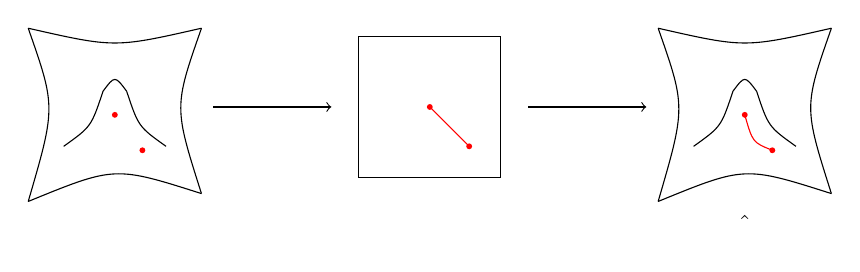
\begin{tikzpicture}
        \draw (-0.1, -0.2) .. controls (1, 0.25) .. (2.1, -0.1);
        \draw (2.1, -0.1) .. controls (1.75, 1) .. (2.1, 2);
        \draw (2.1, 2) .. controls (1, 1.75) .. (-0.1, 2);
        \draw (-0.1, 2) .. controls (0.25, 1) .. (-0.1, -0.2);

        \draw (0.35, 0.5) .. controls (0.7, 0.75) .. (0.85, 1.2);
        \draw (0.85, 1.2) .. controls (1.0, 1.4) .. (1.15, 1.2);
        \draw (1.15, 1.2) .. controls (1.3, 0.75) .. (1.65, 0.5);

        \node[fill, red, circle, inner sep=0.75pt] at (1, 0.9) {};
        \node[fill, red, circle, inner sep=0.75pt] at (1.35, 0.45) {};

        \node at (1, -0.5) {\(\x\)};

        \draw[->] (2.25, 1) -- (3.75, 1);
        \node at (3, 1.25) {\(\fl\)};

        \draw (4.1, 0.1) -- (5.9, 0.1);
        \draw (5.9, 0.1) -- (5.9, 1.9);
        \draw (5.9, 1.9) -- (4.1, 1.9);
        \draw (4.1, 1.9) -- (4.1, 0.1);

        \node[fill, red, circle, inner sep=0.75pt] at (5, 1) {};
        \node[fill, red, circle, inner sep=0.75pt] at (5.5, 0.5) {};

        \draw[red] (5, 1) -- (5.5, 0.5);

        \node at (5, -0.5) {\(\z\)};

        \draw[->] (6.25, 1) -- (7.75, 1);
        \node at (7, 1.25) {\(\re\)};

        \draw (7.9, -0.2) .. controls (9, 0.25) .. (10.1, -0.1);
        \draw (10.1, -0.1) .. controls (9.75, 1) .. (10.1, 2);
        \draw (10.1, 2) .. controls (9, 1.75) .. (7.9, 2);
        \draw (7.9, 2) .. controls (8.25, 1) .. (7.9, -0.2);

        \draw (8.35, 0.5) .. controls (8.7, 0.75) .. (8.85, 1.2);
        \draw (8.85, 1.2) .. controls (9.0, 1.4) .. (9.15, 1.2);
        \draw (9.15, 1.2) .. controls (9.3, 0.75) .. (9.65, 0.5);

        \node[fill, red, circle, inner sep=0.75pt] at (9, 0.9) {};
        \node[fill, red, circle, inner sep=0.75pt] at (9.35, 0.45) {};

        \draw[red] (9, 0.9) .. controls (9.1, 0.55) .. (9.35, 0.45);

        \node at (9, -0.5) {\(\hat{\x}\)};
    \end{tikzpicture}
    \caption{在维度为 \(d = 2\) 的 \(\R^{3}\) 流形上通过流形展平进行插值的描述。要在数据流形上对两点进行插值，首先通过展平映射 \(\fl\) 将它们映射到展平空间，取它们的凸插值，然后通过重建映射 \(\re\) 将它们映射回数据流形。}
    \label{fig:idealized_interpolation}
\end{figure}

\paragraph{通过双层网络的经典尝试。} 正如我们在上面看到的，在 PCA 的情况下，单层线性神经网络就足够了。但对于 NLPCA 来说，情况不再如此。1991 年，Kramer \cite{Kramer1991NonlinearPC} 提出利用具有 sigmoid 激活函数的双层网络的通用表示属性，使用双层神经网络来表示编码器映射 $f$（或其逆映射 $g$），从而解决 NLPCA 问题：
\begin{equation}
    \z = \vW_2 \sigma(\vW_1\x +\vb),
\end{equation}
其中 $\sigma(\spcdot)$ 是 sigmoid 函数：
\begin{equation}
    \sigma(x) = \frac{1}{1+ e^{-x}}.
\end{equation}
Cybenko \cite{Cybenko1989ApproximationBS} 证明了上述形式的函数（具有足够的隐藏节点）可以以任意精度逼近任何平滑的非线性函数，例如编码器 $f(\spcdot)$。特别是，它们可以表示支撑在低维流形并集上的数据分布的展平和重建映射，如\Cref{fig:idealized_interpolation}所示。Kramer 提出的原始网络的整体架构如\Cref{fig:NLPCA}所示。
\begin{figure}[tb]
    \centering
    
\includegraphics[width=0.6\linewidth]{\toplevelprefix/chapters/chapter6/figs/kramer1991nonlinearPCA.png}
    \caption{由 Kramer \cite{Kramer1991NonlinearPC} 提出的非线性 PCA，其编码和解码映射均采用深度为 2 的自联想神经网络。}
    \label{fig:NLPCA}
\end{figure}

不幸的是，与上述 PCA 的情况不同，这些网络的参数 $\boldsymbol{\theta} =
(\vW, \vb)$ 通常没有闭式学习方案。因此，有人提出在重建误差的监督下通过反向传播来训练网络：
\begin{equation}\label{eq:nonlinear-pca-ch5}
    \min_{\boldsymbol{\theta}} \mathbb{E}[ \|\x -
    \hat{\x}(\boldsymbol{\theta})\|_2^2].
\end{equation}
与 PCA 的简单情况相比，我们利用相同的重建目标进行学习，但使用复杂得多的非线性模型类来参数化和学习编码器和解码器。尽管像 Cybenko 这样的通用逼近属性表明，\textit{原则上}通过该框架学习一致的自编码器是可能的——因为对于任何随机数据样本，只要给定足够的参数，这样的自编码对就存在——但人们通常发现使用梯度下降找到它们是非常困难的。
此外，为了获得足够信息量的重建目标并对高维真实世界数据（如图像）的分布进行建模，所需的样本和隐藏节点数量可能非常庞大。
另外，作为学习到的表征紧凑性的度量，瓶颈层 $\z$ 的（较低）维度通常是启发式选择的。\footnote{在后来的工作 \cite{Hinton-1993} 中，Hinton 等人建议使用最小描述长度（MDL）原则来促进学习到的编码方案的紧凑性，其精神与本书中介绍的率失真度量非常相似。}

\paragraph{通过更深的网络进行流形展平。}
基于深度网络的现代实践，众所周知，这种经典的浅而宽的网络架构很难通过反向传播（BP）进行有效且高效的训练，部分原因是 sigmoid 函数的梯度消失问题。因此，现代实践通常建议将非线性变换 $f$（或 $g$）进一步分解为更多层简单变换的组合，从而产生更深的网络架构 \cite{Hinton504}，如\Cref{fig:ccnet_layers}所示。
%在现代背景下，为了在图像等复杂的真实世界数据分布上取得良好的性能，对基本重建成本 \eqref{eq:nonlinear-pca-ch5} 进行进一步的细化也被证明是必要的。

\begin{figure}[htb]
    \centering
    \begin{tikzpicture}
        \draw (-0.1, -0.2) .. controls (1, 0.25) .. (2.1, -0.1);
        \draw (2.1, -0.1) .. controls (1.75, 1) .. (2.1, 2);
        \draw (2.1, 2) .. controls (1, 1.75) .. (-0.1, 2);
        \draw (-0.1, 2) .. controls (0.25, 1) .. (-0.1, -0.2);
        \draw (0.35, 0.5) .. controls (0.7, 0.75) .. (0.85, 1.2);
        \draw (0.85, 1.2) .. controls (1.0, 1.4) .. (1.15, 1.2);
        \draw (1.15, 1.2) .. controls (1.3, 0.75) .. (1.65, 0.5);

        \node at (1, -0.5) {\(\x\)};

        \draw[->] (2.25, 1.25) -- (3.25, 1.25);
        \node at (2.75, 1.5) {\(\fl_{1}\)};

        \draw[->] (3.5, 1.25) -- (4.5, 1.25);
        \node at (4, 1.5) {\(\fl_{2}\)};

        \draw[->] (4.75, 1.25) -- (5.75, 1.25);
        \node at (5.25, 1.5) {\(\cdots\)};

        \draw[->] (6, 1.25) -- (7, 1.25);
        \node at (6.5, 1.5) {\(\fl_{L}\)};

        \draw[->] (7, 0.75) -- (6, 0.75);
        \node at (6.5, 0.5) {\(\re_{L}\)};

        \draw[->] (5.75, 0.75) -- (4.75, 0.75);
        \node at (5.25, 0.5) {\(\cdots\)};

        \draw[->] (4.5, 0.75) -- (3.5, 0.75);
        \node at (4, 0.5) {\(\re_{2}\)};

        \draw[->] (3.25, 0.75) -- (2.25, 0.75);
        \node at (2.75, 0.5) {\(\re_{1}\)};

        \draw (7.3, 0.1) -- (9.1, 0.1);
        \draw (9.1, 0.1) -- (9.1, 1.9);
        \draw (9.1, 1.9) -- (7.3, 1.9);
        \draw (7.3, 1.9) -- (7.3, 0.1);

        \node at (8.2, -0.5) {\(\z\)};

    \end{tikzpicture}
    \caption{展平与重建对 \((\fl, \re)\) 构造过程的示意图，其中编码器 \(\fl =
        \fl_{L} \circ \fl_{L - 1} \circ \cdots \circ \fl_{1}\) 由展平层复合构成，而解码器 \(\re
        = \re_{1} \circ \re_{2} \circ \cdots \circ \re_{L}\) 由每个 \(\fl_{\ell}\) 的逆复合构成。}
    \label{fig:ccnet_layers}
\end{figure}

鉴于像 Cybenko 定理这样的通用近似定理，人们最初可能会想，从概念上讲，为什么更深的自编码器应该比浅层的更受青睐。
纯粹从表达能力的角度来看，我们可以通过与展平非线性流形（我们假设的数据分布支撑其上）任务相关的几何视角来理解这一现象。一种纯粹构造性的展平流形的方法是增量进行的，这与我们在
\Cref{ch:denoising}到\Cref{ch:deep-networks}中看到的扩散、去噪和压缩之间的相互作用相平行。在几何设定中，对应于 $f_{\ell}$ 的增量\textit{展平过程}采取的形式是：将流形上某一点的邻域变换得更接近平坦流形（即子空间），并强制与其余数据样本保持局部一致性；解码器中相应的增量操作 $g_{\ell}$ 则撤销这一变换。这一过程精确地结合了关于底层流形的曲率信息，该信息是从数据样本中估计出来的。给定来自流形的足够样本以及对这一概念过程的精心实例化，就有可能将这一草图实现为一个计算过程，以白盒方式可验证地展平非线性流形 \cite{Psenka-JMLR24}。然而，由于可扩展性不佳，该方法在应用于图像等高维数据分布时受到限制，这促使人们开发更灵活的增量自编码方法。

\subsection{稀疏自编码}
在上述自编码方案中，特征空间的维度 $d$ 通常被选择为远低于原始数据空间的维度 $D$，以便显式地强制或促进学到的表征是低维的。然而，在实践中，我们通常不知道数据分布的内在维度。因此，自编码特征空间维度的选择通常是凭经验进行的。在更一般的情况下，数据分布可能是几个低维子空间或子流形的混合。在这些情况下，不再可能对所有特征一起强制使用单一的低维空间。

稀疏自编码器旨在解决其中的一些局限性。特别是，特征空间的维度可以等于甚至高于数据空间的维度，如
\Cref{fig:SAE} 所示。然而，特征被要求在特征空间中高度稀疏。因此，如果在目标
\eqref{eqn:autoencode-objective-ch5} 中除了降率之外，我们还引入稀疏性作为简约性的度量，我们就会得到稀疏自编码的一个新目标：
\begin{equation}
    \min_{f, g}
    [\|\Z\|_0 - \Delta R_{\epsilon}(\Z) + d(\X, \hat \X)],
    \label{eqn:autoencode-sparse}
\end{equation}
其中 $\ell^0$-“范数” $\|\spcdot\|_0$ 已知可以促进稀疏性。
这与我们在前面的
\Cref{ch:deep-networks} 中用来推导白盒 CRATE 架构的稀疏降率目标
\eqref{eq:sparse-rr} 非常相似。

\begin{figure}
    \centering
    
\includegraphics[width=0.5\linewidth]{\toplevelprefix/chapters/chapter6/figs/SAE_diagram.png}
    \caption{稀疏自编码器（SAE）的示意图，与 \Cref{fig:AE} 中典型自编码器（AE）的对比。}
    \label{fig:SAE}
\end{figure}

作为一种以端到端方式学习自编码对的方法，稀疏自编码在过去已被实践过
\cite{Ranzato2006-oq,10.5555/3042573.3042641}，但几乎所有现代自编码框架都转而基于一种不同的、概率性的自编码框架，我们现在将对其进行研究。

\subsection{变分自编码}\label{sec:vae}

%In the classical conception of autoencoding, following Hinton and Rumelhart
%\cite{Rumelhart1986}, the data distribution plays a very minor role in the
%formulation, despite its centrality to the representation we ultimately
%learn. Indeed, in the naive framework, one hopes that by training a
% deep network
%to reconstruct samples from the data distribution with a suitably configured
%bottleneck for the representation $\vz$, the learned encoders $f$ and $g$ will
%naturally end up corresponding to a compact and structured feature
%representation for the data. This is rarely the case in practice.
一种改进的、更现代的自编码方法至今仍有重要应用，那就是\textit{变分自编码}
\cite{Kingma2013-sb,Kingma2019-zh}。
%We will see how this framework, which trains a variational autoencoder (VAE)
%derived through probabilistic modeling considerations, both generalizes the
%classical autoencoder training (via minimization of the reconstruction loss),
%and stabilizes it with appropriate regularization. Later, we will see how to
%go further and go beyond the black-box nature of the deep networks used
%to represent the encoding and decoding mappings $f$ and $g$.
%
%\subsubsection{Probabilistic Perspective on Autoencoding}
%In the manifold model for the data distribution, the key mathematical objects
%are the \textit{support} of the data distribution, namely the manifold $\cM$,
%and the density of the data on the support, say $p$. When we formulate
%autoencoding from the probabilistic perspective, we often think of the
%high-dimensional input $\vx$ as having a density $p$ with support on
% $\R^D$; one
%can think of adding a very small amount of noise to the (degenerate)
%distribution supported on the manifold $\cM$ to obtain this density
% $p$, in line
%with our denoising-diffusion constructions in \Cref{ch:denoising}.
%Then the goal of generative probabilistic modeling is to learn the density $p$
%from samples $\vx$, say from a class of models $p(\vx;\, \vtheta)$
% parameterized
%by $\vtheta$.
它用概率术语来表述表征学习问题，即寻找一个模型 $p(\vx; \vtheta)$
使其最大化数据样本（或更一般地，总体数据分布）的似然：
\begin{equation*}\label{eq:VAE-MLE}
    \max_{\vtheta}\, \bE_{\vx}[ \log p(\vx;\, \vtheta) ].
\end{equation*}
%For certain representative classes of data distributions $p$ %
%and sufficiently expressive classes of models $p(\vx;\, \vtheta)$, even simpler
%learning problems than maximum likelihood estimation are known to be
%statistically hard \cite{Yang1999-wb}. Hence it is desirable to exploit the
%knowledge that $\vx$ has low-dimensional structure by seeking to factor the
%distribution $p(\vx ;\, \vtheta)$ according to a low-dimensional ``latent''
%variable model $\vz$. Indeed,
通过条件化，我们可以写出 $p(\vx, \vz ;\, \vtheta)
= p(\vz;\, \vtheta) p(\vx \mid \vz;\, \vtheta)$，并且
\begin{align*}
    p(\vx; \vtheta) &= \int p(\vz;\, \vtheta) p(\vx \mid \vz;\,
    \vtheta) \odif \vz
    \\
    &=
    \bE_{\vz \sim p(\,\cdot\,;\, \vtheta)}[ p(\vx \mid \vz;\, \vtheta) ].
\end{align*}
%Classically, our model for the data distribution $p(\vx;\, \vtheta)$
% corresponds
%to a choice of the latent distribution $p(\vz;\, \vtheta)$ and the conditional
%distribution $p(\vx \mid \vz;\, \vtheta)$.
%Even so, computing the model for the data distribution from these latent
%distributions is intractable except in special cases, analogous to those we
%have studied in \Cref{ch:classic-models}.
%By the same token, computing the posterior $p(\vz \mid \vx;\, \vtheta)$ from
%data, allowing us to \textit{encode} samples to their corresponding latents, is
%generally intractable.
%There is hence a trade-off between the expressivity of our generative model,
%its computational tractability, and the accuracy of any approximations we make
%to the underlying probabilistic framework for the sake of
%computational tractability.
%In navigating this trade-off, one also needs a flexible computational approach
%for learning the model parameters $\vtheta$ from data, analogous to the maximum
%likelihood objective.
%
这意味着可以通过\textit{先验} $p(\vz)$ 和条件分布 $p(\vx \mid \vz)$（更一般地对应于解码器）来学习 $\vx$ 的概率模型。
在技术上，贝叶斯法则随后意味着编码所需的\textit{后验} $p(\vz \mid
\vx)$ 可以用先验和解码器（以及 $\vx$ 的样本）来表示，但这在计算上是难以处理的。因此，在 VAE 框架中，我们引入了一个“近似后验”
$q(\vz \mid \vx;\, \veta)$，对应于一个独立的编码器网络，并通过最大化真实似然的下界（称为证据下界，ELBO）来联合学习编码器和解码器，当后验近似紧密时，该下界也是紧密的。
%In the variational autoencoding framework, we
%%navigate this trade-off through three key insights:
%\begin{enumerate}
%\item We posit \textit{simple} distributions for $\vz$ and $\vx$ conditional
%  on $\vz$, but make their parameters depend in a highly flexible way on the
%  input data $\vx$ (where relevant) using deep networks.
%\item We replace the posterior $p(\vz \mid \vx;\, \vtheta)$, used for encoding
%  and whose form is implied (by Bayes rule) by our modeling choices for $\vz$,
%  with a tractable approximation $q(\vz \mid \vx;\, \veta)$, which has its own
%  parameters $\veta$.
%\item We jointly learn $\vtheta$ and $\veta$ via maximizing a tractable lower
%  bound for the likelihood $p(\vx ;\, \vtheta)$, known as the evidence lower
%  bound (ELBO).
%\end{enumerate}

%We will focus on the most useful instantiation of the VAE framework
%in practice, namely
%where the prior $p(\vz ;\, \vtheta)$ and the conditional $p(\vx \mid \vz;\,
%\vtheta)$ are both Gaussian. Namely,
以下实例化在实践中是标准的。我们使用以下高斯分布：
\begin{align*}
    \vz &\sim \cN(\Zero, \vI), \\
    \vx \mid \vz &\sim \cN(g_1(\vz), \diag(e^{g_2(\vz)}) \vI),
\end{align*}
其中 $g = (g_1, g_2)$ 是参数为 $\vtheta$ 的深度网络，对应于自编码器中的\textit{解码器}。
类似地，对于近似后验，我们使用一个高斯分布，其参数由参数为 $\veta$ 的编码器
MLP $f = (f_1, f_2)$ 给出：
\begin{equation*}
    \vz \mid \vx \sim \cN(f_1(\vx), \diag(e^{f_2(\vx)}) \vI).
\end{equation*}
这使得概率编码和解码变得简单：我们只需将数据 $\vx$ 映射到高斯分布的均值和方差参数以进行编码，反之亦然进行解码。
%For learning the encoder and decoder, we start from the maximum likelihood
%objective \Cref{eq:VAE-MLE}, and derive a convenient lower bound known as the
%evidence lower bound, or ELBO. Starting from simple algebraic manipulations
%\begin{align*}
%\log p(\vx;\, \vtheta) &=
%\log \frac{p(\vx, \vz;\, \vtheta)}{p(\vz \mid \vx;\, \vtheta)}
%\\
%&=
%\log \frac{p(\vx, \vz;\, \vtheta)}{q(\vz \mid \vx;\, \veta)}
%+
%\log \frac{q(\vz \mid \vx;\, \veta)}{p(\vz \mid \vx;\, \vtheta)},
%\end{align*}
%we take expectations with respect to $\vz \sim q(\,\cdot\, \mid
%\vx;\, \veta)$ and
%use the Gibbs inequality (\Cref{thm:information-inequality}) to get
%\begin{equation*}
%\log p(\vx;\, \vtheta)
%\geq
%\bE_{\vz \sim q(\,\cdot\, \mid \vx ;\, \veta)} \left[
%  \log \frac{p(\vx, \vz;\, \vtheta)}{q(\vz \mid \vx;\, \veta)}
%\right].
%\end{equation*}
%The right-hand side of this bound is the ELBO; as a lower bound for
% the pointwise
%log-likelihood of $p(\vx;\, \vtheta)$, its maximization offers a
%principled compromise
%between the maximum likelihood objective and computational tractability.
%Interestingly, the derivation above shows that its tightness depends on the KL
%divergence between the approximate posterior $q(\vz \mid \vx;\, \veta)$ and the
%true posterior $p(\vz \mid \vx;\, \vtheta)$, implying that the more
% accurate our
%approximate posterior is, the more maximization of the ELBO leads to
%maximization of the underlying objective of interest, the likelihood of the
%data. Thus,
经过上述操作后，最终的 VAE 目标如下：
%\begin{equation}\label{eq:elbo-objective}
%\max_{\vtheta, \veta}\,
%\bE_{\vx}
%\bE_{\vz \sim q(\,\cdot\, \mid \vx ;\, \veta)} \left[
%  \log \frac{p(\vx, \vz;\, \vtheta)}{q(\vz \mid \vx;\, \veta)}
%\right].
%\end{equation}
\begin{align*}\labelthis\label{eq:elbo-objective}
    &\max_{\vtheta, \veta}\,
    \bE_{\vx}
    \bE_{\vz \sim q(\,\cdot\, \mid \vx ;\, \veta)} \left[
        \log \frac{p(\vx, \vz;\, \vtheta)}{q(\vz \mid \vx;\, \veta)}
    \right]\\
    &\equiv
    \max_{\vtheta, \veta}\,
    \left\{
        2\bE_{\vx}\left[
            \bE_{\vz \sim q(\,\cdot\, \mid \vx ;\, \veta)} \left[
                \log p(\vx \mid \vz;\, \vtheta)
            \right]
            + \ip{ f_2(\vx) - e^{f_2(\vx)}}{\mathbf{1}}
            - \norm{f_1(\vx)}_2^2
        \right]
    \right\}. \labelthis \label{eq:elbo-for-gaussians}
\end{align*}
我们可以将其理解为一个正则化的自编码目标，其中在 ELBO 的第一项中有一个有趣的额外一致性约束。

同时，读者应注意 VAE 形式化过程中做出的许多任意决定（例如，高斯分布的选择和参数化）。这导致了一个复杂的训练目标，尽管经过了十多年的研究，高效优化该目标仍然是一个挑战。最近的表征学习方法对这一基线进行了显著改进，它们甚至可以在我们在 \Cref{ch:deep-networks} 中开发的白盒框架中进行表述，正如我们很快就会看到的那样。

% \yima{Robin and Peter, this is a good place to have some discussion
% about the use of VAE for the latent diffusion (and denoising)
% models, as in SD-VAE. Some of its difficulties become the
% justification for the RAE to be introduced in the next subsection.}

\paragraph{基于 VAE 的潜在扩散}
VAE 的一个重要应用是在潜在扩散模型 \cite{rombach2022high} 的背景下，其中首先训练 VAE 以学习图像等高维数据的更紧凑和规则化的潜在表征。然后可以在潜在空间中训练扩散模型，以获取表征的分布，从而从中生成新样本，如图 \ref{fig:VAE-SD} 所示。
\begin{figure}[t]
    \centering
\includegraphics[width=0.8\linewidth]{chapters/chapter6/figs/VAE-SD.png}
    \caption{\cite{rombach2022high} 工作中的潜在扩散模型示意图，该模型利用变分自编码器（左侧红框）来学习数据 $\x$ 的潜在表征。然后学习一个扩散/去噪模型（中间绿框）来获取表征 $\z$。右侧的模块是关于如何通过（基于文本的）控制信号来控制去噪采样过程，我们将在第 \ref{ch:conditional-inference} 章中对此进行研究。}
    \label{fig:VAE-SD}
\end{figure}
这种方法通过利用学到的潜在空间的高度压缩结构，实现了高质量图像的高效生成。\footnote{许多流行的早期图像或视频生成模型都基于这种潜在扩散框架，正如我们在 \Cref{sub:text-cond} 中进一步详细描述的，以及在 \Cref{ch:applications} 中的实现术语所述。}然而，由于后验坍塌以及平衡 ELBO 中的重建项和正则化项等问题，训练 VAE 可能具有挑战性。此外，VAE 中的高斯后验是应用于每个数据点的，并没有在样本之间学习到联合结构，这可能会严重限制学到的表征的质量。
这些挑战促使了替代方法的发展，例如接下来要介绍的表征自编码器（RAE），旨在解决 VAE 的一些局限性，同时仍为生成建模任务提供有效的潜在表征。

%\subsubsection{VAE Training as Probabilistic Autoencoding}
%
%There is a general methodology for maximizing the ELBO objective in
%\Cref{eq:elbo-objective} using stochastic gradient descent and
% various tractable
%Monte Carlo estimators for the associated gradients. However, the task is
%simpler under the Gaussian assumptions we have made above. In this case, the
%ELBO reads
%\begin{align*}
%&\max_{\vtheta, \veta}\,
%\bE_{\vx}
%\bE_{\vz \sim q(\,\cdot\, \mid \vx ;\, \veta)} \left[
%  \log \frac{p(\vx, \vz;\, \vtheta)}{q(\vz \mid \vx;\, \veta)}
%\right]\\
%=&
%\max_{\vtheta, \veta}\,
%\left\{
%  \bE_{\vx}
%  \bE_{\vz \sim q(\,\cdot\, \mid \vx ;\, \veta)} \left[
%    \log p(\vx, \vz;\, \vtheta)
%  \right]
%  + \frac{d \log(2\pi e)}{2}
%  + \frac{1}{2} \ip{ \bE_{\vx}[f_2(\vx)]}{\mathbf{1}}
%\right\}
%\\
%\equiv &
%\max_{\vtheta, \veta}\,
%\left\{
%  \bE_{\vx}
%  \bE_{\vz \sim q(\,\cdot\, \mid \vx ;\, \veta)} \left[
%    \log p(\vx \mid \vz;\, \vtheta)
%    + \log p(\vz)
%  \right]
%  + \frac{1}{2} \ip{ \bE_{\vx}[f_2(\vx)]}{\mathbf{1}}
%\right\}
%\\
%\equiv &
%\max_{\vtheta, \veta}\,
%\left\{
%  2\bE_{\vx}\left[
%    \bE_{\vz \sim q(\,\cdot\, \mid \vx ;\, \veta)} \left[
%      \log p(\vx \mid \vz;\, \vtheta)
%    \right]
%    + \ip{ f_2(\vx) - e^{f_2(\vx)}}{\mathbf{1}}
%    - \norm{f_1(\vx)}_2^2
%  \right]
%\right\}, \labelthis \label{eq:elbo-for-gaussians}
%\end{align*}
%following \Cref{thm:max_entropy} and the Gaussian entropy
% calculation done in \Cref{app:entropy}, where $\equiv$
%denotes equivalence of optimization objectives (in each case, we remove some
%additive constants that do not change the optimization problem's solutions).
%The remaining term corresponds to the ``autoencoding'' part of the ELBO
%objective: intuitively, it seeks to maximize the likelihood of data
% generated by
%the decoder when the latents $\vz$ are distribited according to the approximate
%posterior (generated by the encoder applied to a data sample $\vx$), which is
%a probabilistic form of autoencoding.
%To see this more directly, consider the special case where the approximate
%posterior concentrates on its mean $f_1(\vx)$, for every $\vx$: this
%is the limit
%where its log-variance $f_{2,i}(\vx) \to -\infty$ for each coordinate
%$i = 1, \dots, d$.
%For simplicity, assume moreover that $g_2(\vx) = \mathbf{1}$, giving
% the decoder
%constant unit variance on each coordinate.
%Then the loss term in question converges to
%\begin{align*}
%\bE_{\vx}
%\bE_{\vz \sim q(\,\cdot\, \mid \vx ;\, \veta)} \left[
%  \log p(\vx \mid \vz;\, \vtheta)
%\right]
%&\to
%\bE_{\vx} \left[
%  \log p(\vx \mid f_1(\vx);\, \vtheta)
%\right]
%\\
%&\equiv
%-\frac{1}{2} \bE_{\vx} \left[
%  \|\vx - g_1\circ f_1(\vx)\|_2^2
%\right].
%\end{align*}
%So with a highly confident encoder, which deterministically maps each sample
%$\vx$ to a single point $f_1(\vx)$ in $\vz$-space, and an isotropic decoder,
%the ``autoencoding'' part of the ELBO maximization problem indeed becomes
%a classical autoencoding objective!\footnote{In the general case where $g_2$ is
%not fixed as $\mathbf{1}$, the reader can verify that the autoencoding term in
%the ELBO objective converges to a \textit{regularized} classical autoencoding
%objective.}
%At the same time, note that this special case is actually excluded by the
%extra terms in \Cref{eq:elbo-for-gaussians}---these effectively correspond to
%regularization terms that discourage the encoder from collapsing.
%The general ELBO loss (\Cref{eq:elbo-objective,eq:elbo-for-gaussians}) is
%therefore a strict generalization of the classical autoencoding reconstruction
%objective (\Cref{eq:nonlinear-pca-ch5}), both in terms of its data
% fidelity term
%and in terms of the inclusion of regularization terms.
%
%\subsubsection{Training a VAE}
%VAEs are typically trained by alternating stochastic gradient ascent
% on the ELBO
%objective (\Cref{eq:elbo-for-gaussians}), given individual samples
%$\vx$ from the
%true data distribution and from $\vz \sim q(\,\cdot\,\mid \vx;\, \veta)$. In
%particular, it is standard to collect and train on many independently-generated
%samples $\vz^{i}$ for each sample $\vx$. To take gradients of
%\Cref{eq:elbo-for-gaussians} with respect to the encoder parameters $\veta$,
%one makes use of the so-called reparameterization trick by writing $\vz \sim
%q(\,\cdot\,\mid \vx;\, \veta)$ as
%\begin{equation*}
%\vz =_{\mathrm{d}} f_1(\vx) + \diag(e^{\tfrac{1}{2}f_2(\vx)}) \vg,
%\quad \vg \sim
%\cN(0, \vI),
%\end{equation*}
%where $=_{\mathrm{d}}$ denotes equality in distribution. Then one can simply
%take many independent standard Gaussian samples $\vg^{i}$ for each data sample
%$\vx$, generate the corresponding samples from the approximate posterior
%$\vz^i$, and compute gradients with respect to $\veta$ using automatic
%differentiation without any issues.

\subsection{联合表征与分布学习}
\label{sec:RAE}

以前用于表征学习的训练自编码对的方法都有一个共同的局限性：它们没有\textit{显式地组织}表征空间 $\vZ$，而只是间接地约束它（例如，通过在稀疏自编码器中强制稀疏性或在 VAE 中强制高斯性）。正如我们在本章开头所暗示的，我们之前（在 \Cref{ch:lossy-compression} 中）已经看到了如何做得更好，即通过最大化降率 $\Delta
R_{\epsilon}(\vZ)$ 同时确保重建一致性来学习表征 $\vZ$。我们将在本节中更详细地描述这一过程，特别是还将演示如何在学到的表征空间 $\vZ$ 中进行\textit{高效采样}。

正如我们在 \Cref{ch:lossy-compression} 末尾（第
\ref{sec:representations-image} 节）所看到的，我们通常可以学习到数据 $\X$ 的良好表征 $\Z$：
\begin{equation}
    f: \X \rightarrow \Z,
\end{equation}
基于一些端到端的监督或自监督方法，包括分别在第 \ref{sec:MCR2-classification} 节和第 \ref{sec:SimDINO} 节中介绍的 MCR$^2$ 和 SimDINO 方法。正如我们还论证过的，这样学到的表征比原始数据分布具有更好的结构。这些表征倾向于是低维线性子空间（或低秩高斯分布）的混合。然而，我们还没有回答如何评估这样学到的表征的好坏的问题。也就是说，我们能否从它们建立一个反向解码器：
\begin{equation}
    g: \Z \rightarrow \hat{\X}
\end{equation}
使得 $\hat \X$ 和 $\X$ 接近？鉴于前面经典自编码器设置的例子，我们应该期望形如 \eqref{eqn:autoencode-objective-ch5} 的目标函数能够起作用——但是应该使用什么样的样本级一致性损失呢？

此外，这些低维（线性）结构仍然嵌入在高维表征空间中。因此，为了使用这样学到的表征，我们还需要能够获取它们的分布。在第 \ref{ch:denoising} 章中，我们了解到去噪是识别并因此获取这种低维表征的通用方法。因此，我们可以通过从随机噪声开始的（学习到的）去噪过程来获取学到的特征的分布：
\begin{equation}
    h: \boldsymbol{G} \rightarrow \Z.
\end{equation}
此外，我们还了解到，如果 $\Z$ 的目标分布可以（近似地）建模为子空间混合或低秩高斯混合，那么它们的最优去噪算子与 Transformer 或 \Cref{ch:deep-networks} 中介绍的 CRATE 中发现的结构具有相似性。

\begin{figure}[t]
    \centering
    
\includegraphics[width=0.6\linewidth]{chapters/chapter6/figs/mental-picture.pdf}
    \caption{为数据 $\X$ 学习自编码表征 $\Z$（上）以及用于获取表征 $\Z$ 的扩散/去噪模型（下）的示意图。}
    \label{fig:RAE}
\end{figure}

因此，总而言之，我们希望为数据 $\X$ 学习一个自编码器，其表征 $\Z$ 可以被轻松获取。具体而言，我们希望学习一个编码器 $f$ 和一个解码器 $g$，使得：
\begin{enumerate}
    \item 表征 $\Z = f(\X)$ 是原始数据 $\X$ 的一致性表征，如 \Cref{def:bidirectional_rep} 所定义。
    \item 结构化表征 $\Z$ 可以近似建模为低维高斯混合，以便我们可以学习一个去噪器，从而从随机高斯噪声 $\boldsymbol{G}$ 中高效地获取 $\Z$ 的分布。
\end{enumerate}
\Cref{fig:RAE} 展示了上述整体过程。

从 \Cref{ch:lossy-compression} 中我们知道，通过优化（无监督的）MCR$^2$ 目标学到的表征 $\Z$ 满足第二个要求，并且可以被视为具有接近子空间混合或低秩高斯混合的结构。通过引入样本一致性目标，我们可以扩展 \Cref{sec:SimDINO} 中的降率（rate reduction）目标，以学习一致性表征：
\begin{equation}
    \min_{f, g}
    [ - \Delta R_{\epsilon}(\Z) + d(\X, \hat \X)],
    \label{eqn:autoencode-consistent}
\end{equation}
其中 $d(\X, \hat \X)$ 是原始数据 $\X$ 和重建数据 $\hat \X = g(\Z)$ 之间相似度的度量。在实践中，由于单独的目标 $\Delta R_{\epsilon}(\Z)$ 已经促进了 $\Z$ 的低维结构，我们可以首先预训练编码器 $f$ 以最大化 $\Delta R_{\epsilon}(\Z)$，然后在固定编码器 $f$ 的情况下学习解码器 $g$ 以最小化重建损失 $d(\X, \hat \X)$。这种两步法已被证明是有效的，正如我们将在 \Cref{ch:applications} 的第 \ref{sec:RAE-implement} 节中看到的那样。

% \yima{下面似乎暗示去噪器网络和上述解码器网络是分开学习的。RAE 是这种情况吗？}
一旦我们学到了这样的一致性表征 $\Z$，我们就可以学习一个去噪器来获取其分布，正如我们在 \Cref{ch:denoising} 中所研究的那样。具体而言，假设我们有一个概率模型 $p(\z)$ 捕捉了学到的表征 $\vZ$ 的（边缘）分布，以及一个初始的标准高斯分布 $\cN(\Zero, \vI)$。我们的目标是学习一个去噪器 $\bar{\z}$，使其将初始分布中的样本迭代去噪为学到的表征的目标分布。这个去噪器可以使用 \Cref{ch:denoising} 中介绍的目标函数进行训练（关于条件去噪器，另见 \Cref{ch:conditional-inference}）。例如，以流匹配（flow matching）的简单情况为例（回顾 \Cref{exercise:implement_denoising_processes} 和 \Cref{sub:sampling_denoising}）。我们可以将去噪器定义为一个由 $\theta$ 参数化的随时间变化的向量场 $\bar{\z}_{\theta}(t, \z_t)$，它随着时间 $t \in [0, 1]$ 将样本从初始分布变换到目标分布。这里，$\z_t$ 是在时间 $t$ 时 $\z_0$ 和 $\z_1$ 之间的插值：
\begin{equation}
    \z_t = (1 - t)\z_0 + t\z_1,
\end{equation}
其中 $\z_0 \sim p(\z)$ 是来自学到的表征分布的样本，而 $\z_1 \sim \cN(\Zero, \vI)$。
去噪器的训练目标可以表示为：
\begin{equation}
    \min_{\theta} \cL_{\mathrm{FM}}(\theta) = \Ex_{\z_0 \sim p(\z), \z_1 \sim
    \cN(\Zero, \vI), t \sim \mathrm{Unif}(0, 1)} \left[
    \norm{\bar{\z}_{\theta}(t,\z_t) - (\z_1 - \z_0)}_2^2 \right].
\end{equation}

% \yima{这里我们需要讨论为从 VAE 学到的特征分布和从 DINO 学到的特征分布学习潜在扩散/去噪模型的区别……一个是低维的，另一个是高得多维度的。两者都在某种程度上是结构化的（高斯），但 DINO 特征显然更具结构性和线性。回顾第 4 章。}

值得注意的是，为通过 VAE 学到的表征与通过 MCR$^2$ 或 SimDINO 等方法学到的表征学习去噪器之间存在差异。正如在 \Cref{sec:vae} 中所讨论的，VAE 表征被强制要求\textit{逐样本}近似高斯后验，并且没有对潜在空间的联合分布进行建模，这使得表征空间的结构性较弱，去噪过程可能更具挑战性。相比之下，通过 MCR$^2$ 或 SimDINO 学到的表征往往具有更明显的线性和低维结构，例如子空间混合或低秩高斯混合（如 \Cref{sec:SimDINO} 所示），这可以促进去噪过程。这种结构特性可以带来更高效、更有效的去噪模型，因为它们能够更好地利用表征空间的底层几何结构。

一旦我们训练好了去噪器，我们就可以使用它通过扩散过程从学到的表征分布中生成新样本，正如我们在 \Cref{ch:denoising} 中所展示的那样。这就完成了具有可获取表征分布的\textit{表征自编码器}（representation autoencoder, RAE）的学习。
在 \Cref{ch:applications}（特别是 \Cref{sec:RAE-implement}）中，我们将看到 RAE 的具体实现及其在图像生成中的应用。

\section{学习自一致表征}
\label{sec:self-consistency}

在前面的章节中，我们研究了允许我们通过（有损）压缩来学习低维分布的方法。正如我们在 \Cref{ch:intro} 中提到并在前几章中展示的那样，机器智能取得的进展在很大程度上依赖于寻找计算上可行且高效的解决方案来实现所需的压缩，这不仅在理论上是可计算或易处理的，而且在实践中是可扩展的：
\begin{equation}
    \mbox{\textbf{可计算}} \;
    \Longrightarrow \; \mbox{\textbf{易处理}} \; \Longrightarrow \;
    \mbox{\textbf{可扩展}}.
\end{equation}
甚至可以说，过去十多年来机器智能取得的巨大进步，在很大程度上归功于可扩展模型和方法的发展，例如通过反向传播训练深度网络。在数以万计的强大 GPU 上，使用数万亿数据点训练的具有数十亿参数的大型模型，在记忆现有知识方面展示了超人类的能力。这使得许多人相信，随着规模的不断扩大，此类模型的“智能”将继续提高。

在我们庆祝这种大型人造机器学习系统的工程奇迹的同时，我们也必须承认，与自然界的智能相比，这种提高机器智能的方法对资源的需求是不必要地庞大的。自然界的智能生物，包括动物和人类，根本无法承受这种暴力的学习解决方案，因为它们必须在能量、空间和时间预算非常有限的情况下运作，并受到许多严格的物理约束。

首先，有强有力的科学证据表明，我们的大脑并不进行全局的端到端反向传播来改进或纠正其预测。相反，神经科学界早就知道，我们的大脑通过局部的闭环反馈（例如预测编码）来纠正错误。这也是早在 20 世纪 40 年代启发诺伯特·维纳（Norbert Wiener）发展反馈控制理论和控制论（Cybernetics）项目的科学基础。

其次，我们在前面的小节中看到，为了学习一致性表征，需要学习一个双向自编码：
\begin{equation}
    \X
    \xrightarrow{\hspace{1mm} \mathcal{E} = f \hspace{1mm}} \Z
    \xrightarrow{\hspace{1mm} \mathcal{D} = g \hspace{1mm}} \hat{\X}.
\end{equation}
它要求通过某种相似度度量 $d(\X, \hat \X)$ 强制观察到的输入数据 $\X$ 和解码后的 $\hat \X$ 接近。在自然界中，动物或人类很少能直接获取真实数据（ground truth）$\X$。例如，我们永远无法直接获取场景中物体的真实 3D 形状、距离或动力学信息。然而，我们都学会了非常准确和高效地估计和预测它们。因此，一个突出的问题是：即使我们不能直接将我们的估计 $\hat \x$ 与真实值 $\x$ 进行比较，我们如何才能学习 $\X$ 的真实分布？正如我们将在本章中看到的，答案同样在于闭环反馈，以及数据分布的低维性。

正如我们从上一章所知，为了确保表征是一致的，我们需要比较生成的 $\hat \X \sim p(\hat\x)$ 和原始的 $\X \sim p(\x)$，至少在分布上是如此。即使我们确实可以获取 $\X$ 和 $\hat \X$，在技术上，计算和最小化两个分布之间的距离也可能存在问题，特别是当分布的支撑集（support）是低维的时候。\Cref{ch:denoising} 中介绍的 KL 散度在两个没有重叠支撑集的分布之间甚至是没有良好定义的。

作为缓解上述计算和最小化两个（低维）分布之间距离困难的早期尝试，人们曾建议通过判别式方法来学习生成器/解码器 $g$ \cite{Tu-2007}。这种思路催生了{\em 生成对抗网络（Generative Adversarial Nets, GAN）} \cite{goodfellow2014generative} 的思想。它引入了一个判别器 $d$（通常由深度网络建模），以辨别生成样本 $\hat \X$ 和真实样本 $\X$ 之间的差异：
\begin{equation}
    \Z \xrightarrow{\hspace{2mm} g(\z,\eta) \hspace{2mm}} \hat \X, \,
    \X \xrightarrow{\hspace{2mm} d(\x, \theta)\hspace{2mm}} \{\mathbf
    0, \mathbf 1\}.
    \label{eqn:GAN}
\end{equation}
有人建议，我们可以尝试通过生成器 $g$ 和判别器 $d$ 之间的{\em 斯塔克尔伯格博弈（Stackelberg game）}来对齐 $\hat \x$ 和 $\x$ 之间的分布：
\begin{equation}
    \max_{\theta}\min_{\eta} \mathbb{E}_{p({\x})}\big[\log
    d(\x,\theta)\big] + \mathbb{E}_{p({\z})}\big[1 - \log
    d(\underbrace{g(\z,\eta)}_{\hat \x \,\sim\, p_g},\theta)\big].
\end{equation}
也就是说，判别器 $d$ 试图最小化真实样本 $\X$ 和生成样本 $\hat \X$ 之间的交叉熵，而生成器 $g$ 则试图做相反的事情。

可以证明，寻找上述斯塔克尔伯格博弈的均衡等价于最小化 {\em Jensen-Shannon 散度（JS 散度）}：
\begin{equation}
    \mathcal{D}_{JS}(p(\x), p_g(\hat \x)) = \mathcal{D}_{KL}\big(p \|
    (p + p_g)/{2}\big) + \mathcal{D}_{KL}\big(p_g \| (p + p_g)/{2}\big).
\end{equation}
请注意，与 KL 散度相比，即使两个分布的支撑集不重叠，JS 散度也是良好定义的。然而，即使在两个高斯分布之间，JS 散度也没有闭式表达式，而 KL 散度则有。此外，由于数据分布是低维的，优化 JS 散度可能是高度病态的（ill-conditioned）。\footnote{如 \cite{arjovsky2017wasserstein} 所示。} 这也许解释了为什么在 GAN 的许多后续变体中通常会使用许多额外的启发式方法。

因此，也有人建议用推土机（Earth Mover, EM）距离或 Wasserstein 距离来代替 JS 散度。\footnote{粗略地说，对于具有潜在不重叠低维支撑集的分布，JS 散度的行为类似于 $\ell^0$-范数，而 EM 距离的行为类似于 $\ell^1$-范数。} 然而，JS 散度和 Wasserstein 距离在两个一般分布之间都只能近似计算。\footnote{例如，Wasserstein 距离要求计算两个分布在所有 1-Lipschitz 函数上的期望的最大差值。} 此外，即使对于高斯分布，JS 散度和 Wasserstein 距离都没有闭式公式。\footnote{（$\ell^1$-范数）Wasserstein 距离可以被具有闭式解的（$\ell^2$-范数）Wasserstein 距离所界定 \cite{salmona2021gromovwasserstein}。然而，正如高维几何中众所周知的那样，随着维度的升高，$\ell^1$-范数和 $\ell^2$-范数在几何和统计特性上会产生显著偏差 \cite{Wright-Ma-2022}。这个界限可能会变得非常松弛。}

如果很难比较数据 $\X$ 和 $\hat \X$ 的分布，那么是否有可能将学到的特征 $\Z$ 与其在编码器 $f$ 下的像 $\hat \Z$ 进行比较：
\begin{equation}
    \X
    \xrightarrow{\hspace{1mm} \mathcal{E} = f \hspace{1mm}} \Z
    \xrightarrow{\hspace{1mm} \mathcal{D} = g \hspace{1mm}} \hat{\X}
    \xrightarrow{\hspace{1mm} \mathcal{E} = f \hspace{1mm}} \hat \Z?
    \label{eqn:closed-autoencoding}
\end{equation}
这引出了{\em 自一致表征（self-consistent representation）}的概念。
\begin{definition}[自一致表征]\label{def:closed_loop}
    给定数据 \(\vX\)，我们将一对函数 \((f \colon \cX \to \cZ, g
    \colon \cZ \to \cX)\) 称为\textit{自一致表征}，使得\textit{特征} \(\vZ =
    f(\vX)\) 是紧凑且结构化的，并且\textit{自编码特征} \(\hat{\vZ} \doteq f \circ g(\vZ)\) 与 \(\vZ\) \textit{接近}。
    \begin{enumerate}
        \item 如果在某种范数下 \(\vZ \approx \hat{\vZ}\) 以高概率成立，我们称其为\textit{样本级}自一致的。
        \item 如果 \(\Law(\vZ) \approx \Law(\hat{\vZ})\)，我们称该表征是\textit{分布级自一致的}。
    \end{enumerate}
\end{definition}

\subsection{基于斯塔克尔伯格博弈的闭环转录}\label{sec:closed-loop-transcription}

我们如何尝试确保学到的表征是自一致的？像往常一样，假设 $\X = \cup_{k=1}^K \X_k$，其中每个样本子集 $\X_k$ 属于一个低维子流形：$\X_k \subset \mathcal{M}_k, k = 1,\ldots, K$。遵循 \Cref{ch:denoising} 中的符号，我们使用矩阵 $\bm \Pi_k(i,i) = 1$ 来表示样本 $i$ 属于类别 $k$ 的隶属关系，否则 $\bm \Pi_k(i,j) = 0$。我们寻求一个从 $\X$ 到最优表征 $\Z = [\z_1, \ldots, \z_N] \subset \mathbb{R}^{d \times N}$ 的连续映射 $f(\cdot,\bm \theta): \x \mapsto \z$：
\begin{equation}
    \bm X  \xrightarrow{\hspace{2mm} f(\x, \bm \theta) \hspace{2mm}} \bm Z,
    \label{eqn:LDR}
\end{equation}
该映射最大化以下编码降率（MCR$^2$）目标：
\begin{equation}\label{eq:mcr2-formulation}
    \begin{split}
        \max_{\Z} \; \Delta R_\epsilon(\Z  \mid \bm{\Pi}) %
        &\doteq \underbrace{\frac{1}{2}\log\det \Big(\I + {\alpha} \Z
        \Z^\top \Big)}_{R_{\epsilon}(\Z)} \;-\;
        \underbrace{\sum_{k=1}^{K}\frac{\gamma_k}{2} \log\det\Big(\I
                + {\alpha_k} \Z \bm{\Pi}^{j} \Z^\top
        \Big)}_{R^c_{\epsilon}(\Z \mid \bm \Pi)},
    \end{split}
\end{equation}
其中对于每个 $k = 1,\dots, K$，$\alpha = {d}/({N\epsilon^2})$，$\alpha_k =
d/({\mathrm{tr}(\bm{\Pi}_k)\epsilon^2})$，$\gamma_k =
{\mathrm{tr}(\bm{\Pi}_{k})}/{N}$。

通过最大化上述目标 \eqref{eq:mcr2-formulation} 来学习这种单边映射 \eqref{eqn:LDR} 的一个问题是，它倾向于扩展每个类别中特征的学到子空间的维度\footnote{如果特征空间 $d$ 的维度过高，最大化降率可能会高估每个类别的维度。因此，为了学习一个好的表征，需要预先为特征空间选择一个合适的维度，正如 \cite{yu2020learning} 的实验中所实现的那样。事实上，即使在最简单的单子空间情况（即经典的 PCA \cite{Jolliffe1986}）中，同样的“模型选择”问题也依然存在。据我们所知，在异构噪声情况下选择正确的主成分数量仍然是一个活跃的研究课题 \cite{hong2020selecting}。}，正如我们在 \Cref{ch:denoising} 的 \Cref{sec:chap4-representation-learning-problem} 中所见。为了验证学到的特征是否一致，即既不高估也不低估内在的数据结构，我们可以考虑学习一个从表征 $\Z =
f(\X,\bm\theta)$ 回到数据空间 $\x$ 的解码器 $g(\cdot,\eta): \z \mapsto  \x$：$\hat \X = g(\Z, \bm\eta)$：
\begin{equation}
    \X \xrightarrow{\hspace{2mm} f(\x, \bm\theta)\hspace{2mm}} \Z
    \xrightarrow{\hspace{2mm} g(\z, \bm \eta) \hspace{2mm}} \hat \X,
    \label{eqn:autoencoding-ch6}
\end{equation}
并检查 $\X$ 和 $\hat \X$ 有多接近。这构成了一个自编码，这正是我们在前面的 \Cref{ch:consistent-representations} 中广泛研究的内容。

\paragraph{在特征空间中测量距离。}
然而，正如我们上面所讨论的，如果我们无法选择计算 $\X$ 和 $\hat \X$ 之间的距离，我们就只能选择比较它们对应的特征 $\Z$ 和 $\hat \Z =
f(\hat \X, \bm \theta)$。请注意，在 MCR$^2$ 目标下，生成的 $\Z$ 或 $\hat \Z$ 的分布倾向于是分段线性的，因此它们的距离可以更容易地计算。更准确地说，由于每个类别的特征 $\Z_k$ 和 $\hat{\Z}_k$ 接近于低维子空间/高斯分布，它们的“距离”可以通过降率来测量，其中 \eqref{eq:mcr2-formulation} 限制在两个大小相等的集合上：
\begin{equation}
    \Delta R_\epsilon\big(\Z_k, \hat{\Z}_k\big) \doteq
    R_\epsilon\big(\Z_k \cup \hat{\Z}_k\big) - \frac{1}{2} \big(
    R_\epsilon\big(\Z_k) + R_\epsilon\big(\hat \Z_k)\big).
\end{equation}
$\Z$ 和 $\hat \Z$ 之间的总距离由下式给出：
\begin{equation}
    d(\Z, \hat \Z) \doteq   \sum_{k=1}^K \Delta R_\epsilon\big(\Z_k,
    \hat{\Z}_k\big) =  \sum_{k=1}^K \Delta R_\epsilon\big(\Z_k,
    f(g(\Z_k, \bm\eta),\bm \theta)\big).
    \label{eqn:Z-distance}
\end{equation}

如果我们有兴趣辨别原始数据 $\X$ 及其解码后的 $\hat \X$ 分布中的{\em 任何}差异，我们可以将特征编码器 $f(\cdot, \bm \theta)$ 视为一个“判别器”，通过简单地最大化距离 $d(\X, \hat \X)$ 来{\em 放大}所有 $\X_k$ 和 $\hat \X_k$ 对之间的任何差异：
\begin{equation}
    \max_f d(\Z, \hat \Z) = \max_{\bm \theta} \sum_{k=1}^K \Delta
    R_\epsilon\big(\Z_k, \hat{\Z}_k\big) = \max_{\bm \theta}
    \sum_{k=1}^K \Delta R_\epsilon\big(f(\X_k,\bm \theta),
    f(\hat{\X}_k,\bm \theta)\big).
    \label{eqn:max-distance}
\end{equation}
也就是说，$\X$ 和 $\hat \X$ 之间的“距离”可以被测量为这两个集合中所有类别对之间可达到的最大降率。在某种程度上，这衡量了解码后的 $\hat \X$ 与原始数据 $\X$ 对齐的好坏程度——从而衡量了编码器 $f$ 的“单射性（injectivity）”的优劣。请注意，这种判别性度量与 GAN \eqref{eqn:GAN} 的思想是一致的，后者试图将 $\X$ 和 $\hat \X$ 分为两类，并通过交叉熵来衡量。

尽管如此，这里的判别式编码器 $f$ 自然地推广到了数据分布是多类和多模态的情况，并且判别性是通过一种更精细的度量——降率——来衡量的，而不是 GAN 中使用的典型二分类损失（例如交叉熵）。也就是说，我们可以将编码器 $f$ 视为一个广义的判别器，它取代了 \eqref{eqn:GAN} 中的二元分类器 $d$：
\begin{equation}
    \Z \xrightarrow{\hspace{2mm} g(\z,\bm \eta) \hspace{2mm}} \hat
    \X, \, \X \xrightarrow{\hspace{2mm} f(\x, \bm
    \theta)\hspace{2mm}} \{\hat \Z, \Z\}.
    \label{eqn:closed-loop-GAN}
\end{equation}
整体流程可以通过以下“闭环”图来说明：
\begin{equation}
    \X \xrightarrow{\hspace{2mm} f(\x, \bm \theta)\hspace{2mm}} \Z
    \xrightarrow{\hspace{2mm} g(\z,\bm \eta) \hspace{2mm}} \hat \X
    \xrightarrow{\hspace{2mm} f(\x, \bm \theta)\hspace{2mm}} \ \hat \Z,
\end{equation}
其中整体模型具有参数：$\bm \Theta = \{\bm \theta,
\bm \eta\}$。\Cref{fig:auto-encoding-closed} 展示了整体过程。

\begin{figure}[t]
    {
\includegraphics[width=1.0\linewidth]{\toplevelprefix/chapters/chapter6/figs/diagrams_redu_gan_2.pdf}}
    \caption{{\bf %
        闭环转录。} 编码器 $f$ 具有双重作用：它通过最大化 $\z$ 的降率来学习数据 $\x$ 的表征 $\z$，同时它也是数据 $\x$ 和解码后的 $\hat \x$ 之间任何差异的“反馈传感器”。解码器 $g$ 也具有双重作用：它是一个纠正 $\x$ 和 $\hat \x$ 之间差异的“控制器”，同时它也旨在最小化学到的表征的总编码率。} \label{fig:auto-encoding-closed}
\end{figure}

\paragraph{作为双人博弈的编码器和解码器。}
显然，为了确保学到的自编码是自一致的，解码器 $g(\cdot, \bm \eta)$ 的主要目标是{\em 最小化} $\Z$ 和 $\hat \Z$ 之间的距离。也就是说，为了学习 $g$，我们希望最小化距离 $d(\Z, \hat \Z)$：
\begin{equation}
    \min_g d(\Z, \hat \Z) \doteq \min_\eta  \sum_{k=1}^K \Delta
    R\big(\Z_k, \hat{\Z}_k\big) =  \min_{\bm \eta}  \sum_{k=1}^K
    \Delta R\big(\Z_k, f(g(\Z_k, \bm \eta),\bm \theta)\big),
    \label{eqn:min-distance}
\end{equation}
其中 $\Z_k = f(\X_k,\bm \theta)$ 且 $\hat \Z_k = f(\hat{\X}_k,\bm\theta)$。

\begin{example}
    人们可能会想，为什么需要$f(\cdot, \bm \theta)$ 通过$\max_{\bm \theta} \Delta R_\epsilon\big(f(\X,\bm
    \theta), f(\hat \X, \bm \theta)\big)$ 来充当 $\X$ 和 $\hat \X$ 之间的判别器。\Cref{fig:decoder} 给出了一个简单的说明：可能存在许多解码器 $g$，使得 $f\circ g$ 是一个恒等（Id）映射。对于特征空间中子空间 $S_{\z}$ 内的所有 $\z$，都有 $f\circ g(\z) = \z $。然而，$g\circ f$ 对于原始分布 $S_{\x}$（为简单起见，这里画成一个子空间）中的 $\x$ 并不一定是一个自编码映射。也就是说，$g\circ f(S_{\x}) \not\subset S_{\x}$，更不用说 $g\circ f(S_{\x}) = S_{\x}$ 或 $g\circ f(\x) = \x$ 了。人们应该预料到，如果不仔细控制 $g$ 的像，这种情况将以高概率发生，特别是当 $\x$ 分布的支撑集在原始高维数据空间中是极低维的时候。
\end{example}
\begin{figure}
    \centering{
\includegraphics[width=3.0in]{\toplevelprefix/chapters/chapter6/figs/diagrams_fig1.pdf}}
    \caption{\textbf{高维空间中低维子流形的{嵌入}。} $S_{\x}$（蓝色）是原始数据 $\x$ 的子流形；$S_{\z}$（红色）是 $S_{\x}$ 在映射 $f$ 下的像，代表学到的特征 $\z$；绿色曲线是特征 $\z$ 在解码\mbox{映射 $g$ 下的像。} } \label{fig:decoder}
\end{figure}

比较 \eqref{eqn:min-distance} 和 \eqref{eqn:max-distance} 在相同距离度量上的收缩（contractive）和对比（contrastive）性质，我们自然地将编码器 $f(\cdot, \bm
\theta)$ 和解码器 $g(\cdot, \bm \eta)$ 的角色视为“{\bf 一场双人博弈}”：{\em 编码器 $f$ 试图放大原始数据与其转录数据之间的差异，而解码器 $g$ 则旨在最小化这种差异。} 现在为了方便起见，让我们定义“闭环编码”函数：
\begin{equation}
    h(\x, \bm \theta,\bm \eta) \doteq f\big(g\big(f(\x, \bm \theta),
    \bm \eta\big), \bm \theta\big): \; \x \mapsto \hat \z.
\end{equation}

理想情况下，我们希望这个函数非常接近 $f(\x, \bm
\theta)$，或者至少它们的像的分布应该是接近的。使用这个符号，结合 \eqref{eqn:min-distance} 和 \eqref{eqn:max-distance}，$\X$ 和 $\hat \X$ 之间“距离”的闭环概念可以计算为以下斯塔克尔伯格博弈（参见 \Cref{sec:minimax}）在降率效用上的{\em 均衡点}：
\begin{equation}
    \mathcal{D}(\X, \hat \X) \doteq  \max_{\bm \theta} \min_{\bm
    \eta} \sum_{k=1}^K \Delta R_\epsilon\big(f(\X_k,\bm \theta),
    h(\X_k,\bm \theta,\bm \eta)\big).
    \label{eq:MCR2-GAN-pair}
\end{equation}

请注意，这仅仅衡量了原始数据（的特征）与其转录版本之间的差异。它并没有衡量表征 $\Z$（或 $\hat \Z$）对于 $\X$（或 $\hat \X$）中多个类别的优劣。为此，我们可以将上述距离与原始的 MCR$^2$ 类型目标 \eqref{eq:mcr2-formulation} 结合起来：即学到的 LDR 的降率 $\Delta
R_\epsilon(\Z)$ 和 $\Delta R_\epsilon(\hat \Z)$
$\Z$ 表示 $\X$ 的特征，$\hat \Z$ 表示解码后的 $\hat \X$ 的特征。请注意，尽管编码器 $f$ 试图 {\em 最大化} 数据 $\X$ 的特征 $\Z$ 的多类编码率衰减，但解码器 $g$ 应该 {\em 最小化} 解码后的 $\hat \X$ 的多类特征 $\hat \Z$ 的编码率衰减。也就是说，解码器 $g$ 试图使用实现良好解码质量所需的最小编码率。

因此，用于学习闭环转录的整体“多类”斯塔克尔伯格博弈（Stackelberg game），命名为 CTRL-Multi，如下所示：
\begin{eqnarray}
    &&\max_{\bm \theta} \min_{\bm \eta} \mathcal{T}_{\X}(\bm \theta,
    \bm \eta) \nonumber \\
    &\doteq& \underbrace{\Delta R_\epsilon\big(f(\X,\bm
    \theta)\big)}_{\text{Expansive encode}} + \underbrace{\Delta
        R_\epsilon\big(h(\X,\bm \theta, \bm
    \eta)\big)}_{\text{Compressive decode}} + \sum_{k=1}^K
    \underbrace{\Delta R_\epsilon\big(f(\X_k,\bm \theta), h(\X_k,\bm
    \theta,\bm \eta)\big)}_{\text{Contrastive encode \& Contractive
    decode}}  \nonumber \\
    &=& \Delta R_\epsilon\big(\Z(\bm \theta) \big) + \Delta
    R_\epsilon\big(\hat \Z(\bm \theta, \bm \eta)\big) + \sum_{k=1}^K
    \Delta R_\epsilon\big(\Z_k(
    \bm \theta), \hat \Z_k(\bm \theta, \bm \eta) \big),
    \label{eq:MCR2-GAN-objective}
\end{eqnarray}
并受限于第一项和第二项的某些约束（上限或下限）。

请注意，如果没有与生成部分 $h$ 相关的项，或者将所有这些项固定为常数，上述目标正是 \Cref{ch:denoising} 中引入的原始 MCR$^2$ 目标。在无监督设置中，如果我们将每个样本（及其数据增强）视为其自己的类，上述公式保持完全相同。类的数量 $k$ 仅仅是独立样本的数量。此外，请注意，上述博弈的目标函数仅依赖于数据 $\X$（的特征），因此可以学习编码器和解码器（参数），而无需采样或匹配任何额外的分布（这在 GAN 或 VAE 中通常是必需的）。

作为一种特例，如果 $\X$ 只有一个类，斯塔克尔伯格博弈将退化为一种特殊的“两类”或“二元”形式，\footnote{因为前两个编码率衰减项自动变为零} 命名为 CTRL-Binary，
\begin{equation}
    \max_{\bm \theta} \min_{\bm \eta} \mathcal{T}^b_{\X}(\bm \theta,
    \bm \eta) \doteq \Delta R_\epsilon\big(f(\X,\bm \theta), h(\X,\bm
    \theta,\bm \eta)\big) = \Delta R_\epsilon\big(\Z(\bm \theta),
    \hat \Z(\bm \theta, \bm \eta)\big),
    \label{eq:MCR2-GAN-objective-binary}
\end{equation}
这是在 $\X$ 和解码后的 $\hat\X$ 之间进行的，通过将 $\X$ 和 $\hat \X$ 视为两个类 $\{\bm 0, \bm 1\}$。请注意，这种二元情况类似于原始 GAN \eqref{eqn:GAN} 的公式。我们的公式没有使用交叉熵，而是采用了一种更精细的编码率衰减度量，如 \Cref{ch:denoising} 所示，这已被证明可以促进学习到的表征的多样性。 %

有时，即使 $\X$ 包含多个类/模式，人们仍然可以将所有类放在一起视为一个类。那么，上述二元目标就是将所有类的联合分布与其解码后的 $\hat \X$ 对齐。这通常是比多类目标 \eqref{eq:MCR2-GAN-objective} 更容易实现的任务，因为它不需要为数据学习更精细的多类 CTRL，正如我们稍后将在实验中看到的那样。请注意，上述公式的一个良好特性是 {\em 目标中的所有量都是根据学习到的特征的编码率衰减来衡量的}（假设特征最终变成子空间高斯分布）。

人们可能会注意到，上述学习框架从反馈控制系统中广泛实践的闭环误差校正中汲取了灵感。闭环机制用于在编码和解码两个网络之间形成一个整体反馈系统，以校正数据 $\x$ 和解码后的 $\hat \x$ 之间分布的任何“误差”。使用控制理论的术语，可以将编码网络 $f$ 视为用于误差反馈的“传感器”，而将解码网络 $g$ 视为用于误差校正的“控制器”。然而，请注意，这里的控制“目标”既不是标量也不是有限维向量，而是一个连续分布——为了使 $\hat \x$ 的分布与数据 $\x$ 的分布相匹配。这通常是一个无限维空间中的控制问题。$f$ 试图建模的子流形的可能微分同胚空间是无限维的 \cite{Lee2002IntroductionTS}。理想情况下，我们希望当传感器 $f$ 和控制器 $g$ 达到最优时，$\x$ 的分布成为闭环的“不动点”，同时 $\z$ 的分布达到紧凑的线性判别表征。因此，极小极大规划 \eqref{eq:MCR2-GAN-objective} 和 \eqref{eq:MCR2-GAN-objective-binary} 也可以解释为误差反馈传感器和误差减小控制器之间的博弈。

剩下的问题是，上述框架是否确实能够学习到给定数据集的良好（自编码）表征？在给出一些正式的理论证明（在下一小节中）之前，我们先展示一些经验结果。

\paragraph{可视化特征 $\Z$ 与解码特征 $\hat \Z$ 的相关性。} 我们可视化了在 MNIST、CIFAR-10 和 ImageNet（10 类）上从多类目标 \eqref{eq:MCR2-GAN-objective} 学习到的 $\Z$ 和 $\hat{\Z}$ 之间的余弦相似度，这表明了 $\hat{\z} = f\circ g(\z)$ 与 $\z$ 的接近程度。\Cref{fig:justifyz=z} 中的结果表明，$\Z$ 和 $\hat{\Z}$ 在每个类内都对齐得非常好。MNIST 的块对角模式比 CIFAR-10 和 ImageNet 的更清晰，因为 CIFAR-10 和 ImageNet 中的图像具有更多样的视觉外观。

\begin{figure}[t]
    \begin{subfigure}[t]{0.3\textwidth}
        \centering
        
\includegraphics[width=\textwidth]{\toplevelprefix/chapters/chapter6/figs/MNIST_MNIST_ZZhat_heatmap_epo200.png}
        \caption{MNIST}
    \end{subfigure}
    \hfill
    \begin{subfigure}[t]{0.3\textwidth}
        \centering
        
\includegraphics[width=\textwidth]{\toplevelprefix/chapters/chapter6/figs/cifar_heatmat_cifar.png}
        \caption{CIFAR-10}
    \end{subfigure}
    \hfill
    \begin{subfigure}[t]{0.3\textwidth}
        \centering
        
\includegraphics[width=\textwidth]{\toplevelprefix/chapters/chapter6/figs/Imagenet_heatmat_epoch200000.png}
        \caption{ImageNet}
    \end{subfigure}
    \caption{{可视化} %
        $\Z$ 和 $\hat{\Z}$ 之间的对齐：(\textbf{a}) MNIST、(\textbf{b})
    CIFAR-10 和~(\textbf{c}) ImageNet-10-Class 在特征空间中的 $|\Z^\top \hat{\Z}|$。}
    \label{fig:justifyz=z}
\end{figure}

\paragraph{可视化数据 $\X$ 与解码后的 $\hat \X$ 的自编码。} 我们在 MNIST、CIFAR-10 和 ImageNet（10 类）上比较了一些具有代表性的 $\X$ 和 $\hat{\X}$，以验证 $\hat \x = g\circ f(\x)$ 与 $\x$ 的接近程度。结果如 \Cref{fig:justify_xhat_equals_x} 所示，可视化是根据训练样本生成的。从视觉上看，自编码的 $\hat \x$ 忠实地捕捉了其各自训练样本 $\x$ 的主要视觉特征，尤其是姿态、形状和布局。对于像 MNIST 这样较简单的数据集，自编码图像几乎与原始图像相同。

\begin{figure}[t]
    \begin{subfigure}[t]{0.3\textwidth}
        \centering
        
\includegraphics[width=\textwidth]{\toplevelprefix/chapters/chapter6/figs/MNIST_MNIST_train_images_epoch200.png}
        \caption{{\small MNIST $\X$}}
    \end{subfigure}
    \hfill
    \begin{subfigure}[t]{0.3\textwidth}
        \centering
        
\includegraphics[width=\textwidth]{\toplevelprefix/chapters/chapter6/figs/cifar_input.png}
        \caption{{\small CIFAR-10 $\X$}}
    \end{subfigure}
    \hfill
    \begin{subfigure}[t]{0.3\textwidth}
        \centering
        
\includegraphics[width=\textwidth]{\toplevelprefix/chapters/chapter6/figs/Imagenet_input.png}
        \caption{{\small ImageNet $\X$}}
    \end{subfigure}

    \begin{subfigure}[t]{0.3\textwidth}
        \centering
        
\includegraphics[width=\textwidth]{\toplevelprefix/chapters/chapter6/figs/MNIST_MNIST_train_recon_images_epoch200_multi.png}
        \caption{{\small MNIST $\hat{\X}$}}
    \end{subfigure}
    \hfill
    \begin{subfigure}[t]{0.3\textwidth}
        \centering
        
\includegraphics[width=\textwidth]{\toplevelprefix/chapters/chapter6/figs/cifar_reconstruct.png}
        \caption{{\small CIFAR-10 $\hat{\X}$}}
    \end{subfigure}
    \hfill
    \begin{subfigure}[t]{0.3\textwidth}
        \centering
        
\includegraphics[width=\textwidth]{\toplevelprefix/chapters/chapter6/figs/Imagenet_reconstruct.png}
        \caption{{\small ImageNet $\hat{\X}$}}
    \end{subfigure}
    \caption{在 MNIST、CIFAR-10 和 ImageNet 上可视化学习到的闭环转录的自编码特性 \mbox{($\x \approx \hat{\x} = g\circ
        f(\x)$)}（放大以获得更好的视觉效果）。}
    \label{fig:justify_xhat_equals_x}
\end{figure}

\subsection{低维高斯混合模型}

在上文中，我们已经论证了将学习数据分布的问题表述为闭环自编码问题是可能的。我们还在经验上看到这种方案似乎是有效的。剩下的问题是这种方案何时以及为什么有效。对于具有任意数据分布的最一般情况，很难回答这个问题。然而，像往常一样，让我们看看是否能为数据分布是低维子空间或低秩高斯混合的理想情况得出严格的证明。对这一重要特例的清晰刻画和理解将为更一般的情况提供启示。\footnote{因为大多数具有低维结构的分布都可以被该分布族很好地近似。}

为此，让我们首先假设 \(\vX\) 服从低维高斯混合分布，并且 \(\vX\) 的标签（即子空间分配）由 \(\vy\) 给出。然后，让我们建立一个极小极大优化问题来学习数据分布，例如通过学习将 \(\vX\) 编码为支撑在 \textit{正交} 子空间混合上的表征 \(\vZ\)，以及将 \(\vZ\) 解码回 \(\vX\)。那么，我们想要实现的表征可以通过前面讨论的信息增益版本来最大化，即 \( \Delta R_{\epsilon}(\vZ) = R_{\epsilon}(\vZ) - \sum_{k=1}^K R_{\epsilon}(\bm Z_k) \)，这强制每个类 \(k\) 的表征 \(\vZ_{k}\) 张成一个与其他类的支撑子空间正交的子空间。衡量解码一致性的方法与之前一样，由 \(\sum_{k = 1}^{K}\Delta R_\epsilon(\vZ_{k}, \hat{\vZ}_{k})\) 给出，这强制每个类 \(k\) 的表征 \(\vZ_{k}\) 及其自编码 \(\hat{\vZ}_{k}\) 张成相同的子空间。因此，我们可以建立一个简化的斯塔克尔伯格博弈：
\begin{equation}\label{eq:ctrl_msp_game}
    \max_{\bm \theta}\min_{\bm \eta}\bc{\Delta R_\epsilon(\vZ(\bm
        \theta)) + \sum_{k = 1}^{K}\Delta R_\epsilon(\vZ_{k}(\bm \theta),
    \hat{\vZ}_{k}(\bm \theta, \bm \eta))}
\end{equation}
请注意，这比实践中使用的设置更简单——例如，没有 \(\Delta R_\epsilon(\hat{\vZ})\) 项，并且我们在带有类标签的监督设置中工作（尽管用于证明以下结果的技术很容易扩展到无监督公式）。此外，表征的一致性仅通过 \(\Delta R_\epsilon\) 在分布意义上进行衡量（尽管如果需要，这可以用样本级距离度量（如 \(\ell_{2}\) 范数）来替代，并且可以得出等效的结论，\textit{作必要的修正}）。

在温和的条件下，为了实现所需的编码器和解码器，从而从已经服从相关低维高斯混合分布的数据源 \(\vX\) 中实现 \(\vZ\)，我们只需要一个线性编码器和解码器来解耦和白化高斯分布。然后，我们在 \(\bm \theta\) 和 \(\bm \eta\) 参数化算子范数受限的矩阵的情况下研究此设置。

我们想了解在这种设置下学习到了什么样的最优解。对于这种博弈，一个合适的解概念是 \textit{斯塔克尔伯格均衡}（Stackelberg equilibrium），其中解码器跟随编码器，解码器的最优解完全相对于编码器来定义（而不是特别相对于解码器的某些其他内在属性）。 %
也就是说，在这样的均衡下，解码器应该优化其目标；同时，编码器应该优化其目标，前提是无论它选择什么，解码器都会选择一个最优响应（这可能会影响编码器目标）。用博弈论的术语来说，这就像解码器 \textit{后手} 行动：它在编码器之后选择其权重，并且编码器和解码器都试图据此优化它们的目标。通过 \textit{交替优化}（alternating optimization）的梯度方法来学习序贯均衡在计算上是易于处理的，其中双方使用不同的学习率。对序贯均衡的详细阐述超出了本书的范围，我们在 \Cref{sec:minimax} 中提供了更多技术细节。在这种设置下，我们有以下结果：
\begin{theorem}[\cite{pai2022pursuit}, 节选]\label{thm:ctrl_theory}
    假设 \(\vX\) 分布在子空间的混合上。在某些现实但技术性的条件下，\eqref{eq:ctrl_msp_game} 的所有序贯均衡都服从：
    \begin{itemize}
        \item \(\vZ_{k}\) 位于正交子空间上，并且在这些子空间上是各向同性的，即最大化信息增益。
        \item 自编码是自洽的，即对于所有 \(k\)，\(\vZ_{k}\) 和 \(\hat{\vZ}_{k}\) 张成的子空间是相同的。
    \end{itemize}
\end{theorem}
如果对数据只有几何假设，即没有统计假设，这种自洽性概念是人们所能期望的最好的结果。如果我们假设 \(\vX\) 的列是从低秩高斯混合模型中提取的，那么该定理的类似版本证明了 \(\vZ_{k}\) 也是低秩高斯分布，例如其协方差是各向同性的。 %
本质上，这一结果通过子空间上高斯混合的简单情况验证了，优化信息增益和自洽性的极小极大博弈可以达到最优解。

\section{连续学习自洽表征}
\label{sec:continuous}

\subsection{类增量学习}
\label{sec:class-wise-incremental}

正如我们所见，深度神经网络在判别和生成环境中都展示了为成百上千类对象学习表征的强大能力。然而，网络通常必须离线训练，同时使用从所有类中均匀采样的数据。众所周知，当（开环）网络在没有旧类数据的情况下更新以学习新类时，先前学到的知识将成为 {\em 灾难性遗忘}（catastrophic forgetting）问题的牺牲品 \cite{McCloskey1989catastrophic}。这在神经科学中被称为稳定性-可塑性困境（stability-plasticity dilemma）：确保神经系统能够从新环境中学习，同时保留以前环境中的基本知识的挑战 \cite{Grossberg1987CompetitiveLF}。

相比之下，自然神经系统（例如动物大脑）似乎根本不会遭受这种灾难性遗忘。它们能够发展对新对象的新记忆，同时保留对先前学习对象的记忆。这种能力，无论是对于自然神经系统还是人工神经系统，通常被称为 {\em 增量学习}（incremental learning）、{\em 持续学习}（continual learning）、{\em 序贯学习}（sequential learning）或 {\em 终身学习}（lifelong learning）\cite{controlled-forgetting}。

尽管最近的许多工作强调了如何以更灵活的方式训练人工神经系统，但目前为解决人工神经网络的稳定性-可塑性困境所做的最有力尝试通常需要存储原始样本 \cite{icarl,chaudhry2019tiny} 或提供外部机制 \cite{EWC}。原始样本，特别是在图像等高维输入的情况下，成本高昂且难以扩展，而外部机制——通常包括用于生成回放的辅助网络和表征空间、网络资源的增量分配、网络复制或显式隔离网络的已用和未用部分——需要启发式方法并会产生隐藏成本。

在这里，我们对类似于自然的增量学习设置感兴趣。它以两个关键特性对抗这些现有实践。
\begin{enumerate}
    \item 首先，它应该是 \emph{基于记忆的（memory-based）。} 在学习新类时，没有旧类的原始样本可用于与新数据一起训练网络。这意味着人们必须依赖为旧类学习的紧凑且结构化的“记忆”，例如增量学习的旧类生成表征，以及相关的编码和解码映射 \cite{fearnet}。
    \item 其次，它应该是 \emph{自包含的（self-contained）。} 增量学习发生在一个具有固定容量的单一神经系统中，并且在一个公共表征空间中。最小化遗忘的能力隐含在优化整体学习目标中，而不需要外部网络、架构修改或资源分配机制。
\end{enumerate}

不同类特征的不相干线性结构非常类似于动物大脑下颞叶皮层不同区域中对象的编码方式 \cite{Chang-Cell-2017,Bao2020AMO}。闭环转录 $\X \rightarrow \Z \rightarrow \hat{\X} \rightarrow \hat{\Z}$ 也类似于普遍假设的记忆形成机制 \cite{2020Vandeven,Josselyn2020MemoryER}。这就引出了一个问题：既然大脑中的记忆是以增量方式形成的，那么上述闭环转录框架是否也能支持增量学习？

\paragraph{LDR 记忆采样与回放。} LDR 简单的线性 {\em 结构} 使其特别适合增量学习：每个先前学习类的特征 $\Z_j$ 的分布可以由特征空间中的主子空间 $\mathcal{S}_j$ 显式且简洁地表示。为了保留旧类 $j$ 的记忆，我们在学习新类时只需要保留该子空间。为此，我们只需沿着其前 $r$ 个主成分在子空间上采样 $m$ 个具有代表性的原型特征，并将这些特征表示为 $\Z_{j,old}$。由于 LDR 的简单线性结构，我们可以在学习类 $j$ 后通过计算 $\Z_{j,old}$ 的均值和协方差来从 $\Z_{j,old}$ 中采样。所需的存储空间极小，因为我们只需要存储均值和协方差，并根据需要从中采样。假设到目前为止已经学习了总共 $t$ 个旧类。如果在学习新类时能够保留所有这些类的原型特征（表示为 $\Z_{old} \doteq [\Z^1_{old},\ldots, \Z^t_{old}]$），那么代表过去记忆的子空间 $\{\mathcal{S}_j\}_{j=1}^t$ 也将被保留。关于采样以及计算均值和协方差的详细信息可以在 \cite{tong2023incremental} 的工作中找到。

\begin{figure*}[t]
    \centering
    
\includegraphics[width=0.9\textwidth]{\toplevelprefix/chapters/chapter6/figs/framework-v7.png}
    \caption{用于结构化 LDR 记忆的基于闭环转录的增量学习的\textbf{整体框架}。只需要一个单一的、完全自包含的编码-解码网络：对于新的数据类 $\X_{new}$，新的 LDR 记忆 $\Z_{new}$ 作为编码器和解码器之间的极小极大博弈被增量学习，其约束条件是过去类的旧记忆 $\Z_{old}$ 通过闭环转录（或回放）保持完整：$\Z_{old} \approx \hat{\Z}_{ old} = f(g(\Z_{ old}))$。
    \vspace{-0.2in}}
    \label{fig:framework}
\end{figure*}

\paragraph{带有旧记忆约束的增量学习 LDR。} 请注意，利用学习到的自编码 \eqref{eqn:autoencoding-ch6}，人们可以回放并使用与记忆特征相关的图像（例如 $\hat\X_{old} = g(\Z_{old}, \bm \eta)$），以避免在学习新类时发生遗忘。这通常是生成模型在先前的增量学习方法中的使用方式。然而，在闭环框架下，显式地从特征中回放图像是不必要的。过去的记忆可以通过完全在特征本身上进行优化来有效地保留。

考虑增量学习一类新对象的任务。\footnote{当然，人们也可以考虑更一般的设置，即任务包含一小批新类，而无需进行重大修改。} 我们将相应的新样本集表示为 $\X_{new}$。$\X_{new}$ 的特征表示为 $\Z_{new}(\bm \theta) = f(\X_{new}, \bm \theta)$。我们将它们与旧类的原型特征 $\Z_{old}$ 拼接在一起，形成 $\Z = [\Z_{new}(\bm \theta), \Z_{old}]$。我们将所有特征回放的图像表示为 $\hat{\X} = [{\hat{\X}_{new}(\bm \theta,\bm \eta)}, {\hat{\X}_{old}(\bm \eta)}]$，尽管我们实际上不需要显式地计算或使用它们。我们只需要回放图像的特征，表示为 $\hat{\Z} = f(\hat{\X}, \bm \theta) = [{\hat{\Z}_{new}(\bm \theta,\bm \eta)}, {\hat{\Z}_{old}(\bm \theta,\bm \eta)}]$。

呼应多类 CTRL 目标 \eqref{eq:MCR2-GAN-objective} 的动机，我们希望新类 $\Z_{new}$ 的特征与所有旧类 $\Z_{old}$ 的特征不相干。由于 $\Z_{new}$ 是唯一需要学习其特征的新类，目标 \eqref{eq:MCR2-GAN-objective} 退化为 $k=1$ 的情况：
\begin{equation}
    \min_{\bm \eta} \max_{\bm \theta} \Delta{R_\epsilon(\Z)} +
    \Delta{R_\epsilon(\hat{\Z})}+\Delta{R_\epsilon(\Z_{new},\hat{\Z}_{new})}.
    \label{eqn:unconstrained-minimax}
\end{equation}
然而，当我们更新网络参数 $(\bm \theta,\bm \eta)$ 以优化新类的特征时，更新后的映射 $f$ 和 $g$ 也会改变旧类的特征。因此，为了最小化旧类表征的失真，我们可以尝试强制 $\mbox{Cov}(\Z_{j,old}) = \mbox{Cov}(\hat{\Z}_{j,old})$。换句话说，在学习新类时，我们强制旧类的记忆通过转录循环保持“自洽”：
\begin{equation}
    \Z_{old} \xrightarrow{\hspace{2mm} g(\z,\bm \eta) \hspace{2mm}}
    \hat \X_{old} \xrightarrow{\hspace{2mm} f(\x, \bm
    \theta)\hspace{2mm}} \ \hat \Z_{old}.
\end{equation}
在数学上，这等价于设置
$$\Delta R_\epsilon(\Z_{old},\hat{\Z}_{old}) \doteq  \sum_{j=1}^t
\Delta R_\epsilon(\Z_{j,old},\hat{\Z}_{j,old}) = 0.$$
因此，上述极小极大规划 \eqref{eqn:unconstrained-minimax} 被修改为 {\em 约束} 极小极大博弈，我们将其称为 {\em 增量闭环转录}（incremental closed-loop transcription, i-CTRL）。
该博弈的目标与标准多类 CTRL 目标 \eqref{eq:MCR2-GAN-objective} 相同，但仅包含一个额外的约束：
\begin{eqnarray}
    \min_{\bm \eta} \max_{\bm \theta}
    &&\Delta{R_\epsilon(\Z)}+\Delta{R_\epsilon(\hat{\Z})}+\Delta{R_\epsilon(\Z_{new},\hat{\Z}_{new})}
    \nonumber\\
    && \mbox{subject to} \quad  \Delta R(\Z_{old},\hat{\Z}_{old}) = 0.
    \label{eqn:constrained-minimax}
\end{eqnarray}

在实践中，约束极小极大规划可以通过在编码器 $f(\cdot, \bm \theta)$ 和解码器 $g(\cdot, \bm \eta)$ 之间进行 {\em 交替} 最小化和最大化来求解，如下所示：
\begin{eqnarray}
    &\max_{\bm \theta}
    &\scalebox{0.87}{$\displaystyle\Delta{R_\epsilon(\Z)}\!+\!\Delta{R_\epsilon(\hat{\Z})}\!+\!\lambda\cdot
    \Delta{R_\epsilon(\Z_{new},\hat{\Z}_{new})} - \gamma\cdot
    \Delta{R_\epsilon(\Z_{old},\hat{\Z}_{old})}$}, \label{eqn:relaxed-max}\\
    &\min_{\bm \eta}
    &\scalebox{0.87}{$\displaystyle\Delta{R_\epsilon(\Z)}\!+\!\Delta{R_\epsilon(\hat{\Z})}\!+\!\lambda\cdot
    \Delta{R_\epsilon(\Z_{new},\hat{\Z}_{new})} + \gamma\cdot
    \Delta{R_\epsilon(\Z_{old},\hat{\Z}_{old})}$}; \label{eqn:relaxed-min}
\end{eqnarray}
其中 \eqref{eqn:constrained-minimax} 中的约束 $\Delta R_\epsilon(\Z_{old},\hat{\Z}_{old}) = 0$ 已被转换（并松弛）为具有相应系数 $\gamma$ 和符号的拉格朗日项。我们另外引入了另一个系数 $\lambda$，用于对与新数据相关的编码率衰减项进行加权。

\paragraph{通过增量复习实现联合最优记忆。}
正如我们将看到的，上述约束极小极大规划已经可以实现增量学习的最先进性能。然而，为 {\em 所有类} 开发最优记忆不能仅仅依赖于优雅的遗忘。即使对于人类来说，如果一个对象类只学习一次，随着我们继续学习新类，我们应该预期学到的记忆会消退，除非可以通过复习旧对象类来巩固记忆。 %

为了模拟记忆形成的这一阶段，在增量学习整个数据集之后，我们可能会回过头来再次复习所有类，一次一个类。我们将遍历所有类一次称为一个复习“周期（cycle）”。\footnote{以区别于传统联合学习设置中使用的术语“轮次（epoch）”。} 如果需要，可以进行多个复习周期。复习可以改善学习到的（LDR）记忆，这是完全在预料之中的。但有些令人惊讶的是，闭环框架甚至允许我们以“类无监督（class-unsupervised）”的方式进行复习：在复习旧类（例如 $\X_j$）的数据时，系统不需要类标签，可以简单地将 $\X_j$ 视为新类 $\X_{new}$。也就是说，系统在没有任何修改的情况下优化相同的约束极小极大规划 \eqref{eqn:constrained-minimax}；在系统优化之后，人们可以识别由 $\Z_{new}$ 张成的新学习的子空间，并使用它来替换旧子空间 $\mathcal{S}_j$ 或与之合并。正如我们的实验所示，这种类无监督的增量复习过程可以逐渐提高 LDR 记忆的判别和生成性能，最终收敛到联合学习记忆的性能。

\paragraph{实验验证。}
我们在以下数据集上展示了一些实验结果：MNIST
\cite{lecun1998gradient} 和 CIFAR-10 \cite{krizhevsky2014cifar}。所有实验均在更具挑战性的类增量学习（class-IL）设置下进行。对于 MNIST 和 CIFAR-10，10 个类别被分为 5 个任务（每个任务 2 个类别）或 10 个任务（每个任务 1 个类别）。对于编码器 $f$ 和解码器 $g$，我们采用了一种非常简单的网络架构，该架构修改自 DCGAN \cite{radford2016unsupervised}，仅仅是一个{\em 四层}卷积网络。这里我们仅展示一些定性的视觉结果；更多实验和分析可以在文献 \cite{tong2023incremental} 中找到。

\paragraph{自编码特性的可视化。}
我们首先定性地可视化 MNIST 和 CIFAR-10 上的一些代表性图像 $\X$ 及其对应的重放图像 $\hat{\X}$。模型在数据集被分为 5 个任务的情况下进行增量学习。结果如 \Cref{fig:justify_xhat_equals_x_incremental} 所示，我们观察到重建的 $\hat{\X}$ 保留了 $\X$ 的主要视觉特征，包括形状和纹理。对于像 MNIST 这样较简单的数据集，重放的 $\hat{\X}$ 几乎与输入 $\X$ 完全相同！这是相当了不起的，因为：（1）我们的方法并不像大多数自编码方法那样显式地强制单个样本满足 $\hat{\x} \approx \x$；（2）在增量学习了所有类别之后，生成器并没有忘记如何生成早期学习的数字，例如 0、1、2。对于像 CIFAR-10 这样更复杂的数据集，我们也展示了良好的视觉质量，忠实地捕捉了每张图像的本质。

\begin{figure}[t]
    \begin{subfigure}[t]{0.20\textwidth}
        \centering
        
\includegraphics[width=\textwidth]{\toplevelprefix/chapters/chapter6/figs/mnist_x.png}
        \caption{MNIST $\X$}
    \end{subfigure}
    \hfill
    \begin{subfigure}[t]{0.20\textwidth}
        \centering
        
\includegraphics[width=\textwidth]{\toplevelprefix/chapters/chapter6/figs/mnist_recon_x.png}
        \caption{MNIST $\hat{\X}$}
    \end{subfigure}
    \hfill
    \begin{subfigure}[t]{0.20\textwidth}
        \centering
        
\includegraphics[width=\textwidth]{\toplevelprefix/chapters/chapter6/figs/cifar10_x.png}
        \caption{CIFAR-10 $\X$}
    \end{subfigure}
    \hfill
    \begin{subfigure}[t]{0.20\textwidth}
        \centering
        
\includegraphics[width=\textwidth]{\toplevelprefix/chapters/chapter6/figs/cifar10_x_recon.png}
        \caption{CIFAR-10 $\hat{\X}$}
    \end{subfigure}
    \caption{\small 学习到的自编码特性的可视化（$\hat{\X} = g\circ f(\X)$）。 }
    \label{fig:justify_xhat_equals_x_incremental}
\end{figure}

\paragraph{学习到的特征的主子空间。}
大多数基于生成记忆的方法利用自编码器、VAE 或 GAN 进行重放。每个类别的学习特征 $\Z_j$ 在特征空间中的结构或分布是不清楚的。另一方面，LDR 记忆的特征 $\Z_j$ 具有清晰的线性结构。\Cref{fig:cifar_10_pca_sampling_main} 可视化了所有学习特征之间的相关性 $|\Z^\top\Z|$，我们在两个数据集上都观察到了清晰的块对角模式。\footnote{请注意，这些模式与来自下颞叶皮层不同区域的物体类别响应分布的相似性矩阵非常相似，如 \cite{Bao2020AMO} 的扩展数据图 3 所示。} 这表明不同类别的特征 $\Z_j$ 确实位于彼此不相干的子空间上。因此，每个类别的特征都可以很好地建模为特征空间中的一个主子空间。 %

\begin{figure}[tb]
    \centering
    
\includegraphics[height=4.1cm]{\toplevelprefix/chapters/chapter6/figs/Heatmap_MNIST.jpg}
    
\includegraphics[height=4cm]{\toplevelprefix/chapters/chapter6/figs/Heatmap_CIFAR10.png}
    \caption{\small MNIST（左）和 CIFAR-10（右）在特征空间中 $|\Z^\top \Z|$ 的块对角结构。}
    \label{fig:cifar_10_pca_sampling_main}
\end{figure}

\paragraph{来自主成分样本的重放图像。}
由于每个类别的特征都可以建模为一个主子空间，我们进一步可视化了这些子空间中的各个主成分。\Cref{fig:pca_sampling_main} 分别展示了在 MNIST 和 CIFAR-10 上，沿着不同类别的前 4 个主成分采样特征重放的图像。每一行代表沿着一个主成分的样本，它们清楚地显示出相似的视觉特征，但与其他行中的样本截然不同。我们看到，在学习了所有剩余类别之后，模型记住了“4”的不同姿态。对于 CIFAR-10，增量学习的记忆记住了马和船的代表性姿态和形状。

\begin{figure}[t]
    \begin{subfigure}[t]{0.20\textwidth}
        \centering
        
\includegraphics[width=\textwidth]{\toplevelprefix/chapters/chapter6/figs/mnist_4.png}
        \caption{“4”的采样 $\hat{\x}_{old}$}
    \end{subfigure}
    \hfill
    \begin{subfigure}[t]{0.20\textwidth}
        \centering
        
\includegraphics[width=\textwidth]{\toplevelprefix/chapters/chapter6/figs/mnist_7.png}
        \caption{“7”的采样 $\hat{\x}_{old}$}
    \end{subfigure}
    \hfill
    \begin{subfigure}[t]{0.20\textwidth}
        \centering
        
\includegraphics[width=\textwidth]{\toplevelprefix/chapters/chapter6/figs/horse_z.jpg}
        \caption{“horse”的采样 $\hat{\x}_{old}$}
    \end{subfigure}
    \hfill
    \begin{subfigure}[t]{0.20\textwidth}
        \centering
        
\includegraphics[width=\textwidth]{\toplevelprefix/chapters/chapter6/figs/ship_z.jpg}
        \caption{“ship”的采样 $\hat{\x}_{old}$}
    \end{subfigure}
    \caption{\small 对于 {MNIST}（类别“4”和类别“7”）和 {CIFAR-10}（类别“horse”和“ship”），从距离学习特征的（前 4 个）主成分最近的 $\z$ 重建的 5 个 $\hat \x=g(\z)$ 的可视化。}
    \label{fig:pca_sampling_main}
\end{figure}

\paragraph{增量复习的有效性。}
我们验证了如何通过前面描述的无监督增量复习阶段进一步巩固增量学习的 LDR 记忆。实验在 CIFAR-10 上进行，共 10 个步骤。\Cref{fig:memory_review} 左图展示了在完成所有十个类别的增量学习结束时，第一个类别“airplane”的重放图像，这些图像是沿着前 3 个主成分采样的——每两行（16 张图像）沿着一个主方向。它们的视觉质量仍然非常不错——我们几乎没有观察到遗忘。右图展示了复习一次第一个类别后的重放图像。我们注意到复习后视觉质量有了显著提升，并且子空间中特征的主成分开始对应于同一类别内截然不同的视觉属性。

\begin{figure}
    \centering
    
\includegraphics[width=0.41\textwidth]{\toplevelprefix/chapters/chapter6/figs/memory_before_review_clip.png}
    
\includegraphics[width=0.4\textwidth]{\toplevelprefix/chapters/chapter6/figs/memory_after_review_clip.png}
    \caption{\small CIFAR-10 中类别 1-“airplane”在一次复习周期之前（左）和之后（右）的重放图像 $\hat{\x}_{old}$ 的可视化。}
    \label{fig:memory_review}
\end{figure}

\subsection{样本级连续无监督学习}
\label{sec:sample-wise-incremental}

众所周知，闭环 CTRL 公式即使在没有类别信息的情况下，也可以通过 CTRL-Binary 规划学习到一个不错的自编码：
\begin{align}
    \max_{\bm \theta} \min_{\bm \eta} \quad \Delta R_\epsilon(\Z, \hat{\Z})
    \label{eqn:CTRL-Binary}
\end{align}
然而，请注意 \eqref{eqn:CTRL-Binary} 在实践中是受限的，因为它仅在分布层面上对齐数据集 $\X$ 和重新生成的 $\hat \X$。
无法保证每个样本 $\x$ 都会接近解码后的 $\hat \x = g(f(\x))$。

\paragraph{无监督转录的样本级约束。}
\label{sec:constraints}
为了提高在无监督设置下学习到的表征的判别和生成特性，我们为上述 CTRL-Binary 最大最小博弈 \eqref{eqn:CTRL-Binary} 提出了两种额外的机制。为了简单和统一，这里将它们表述为关于降率度量的等式约束，但在实践中，它们可以在优化过程中被软性地强制执行。

\paragraph{通过闭环转录实现样本级自洽性。}
首先，为了解决 CTRL-Binary 无法学习到样本级一致的自编码的问题，我们需要促使每个样本的 $\hat \x$ 接近 $\x$。在 CTRL 框架中，这可以通过强制它们对应的特征 $\z=f(\x)$ 和 $\hat \z = f(\hat \x)$ 接近来实现。
为了促进样本级自洽性，即 $\hat{\x} = g(f(\x))$ 接近 $\x$，我们希望对于所有 $N$ 个样本，$\z$ 和 $\hat{\z}$ 之间的距离为零或很小。
这个距离可以通过降率来衡量：
\begin{align}
    \sum_{i\in N} \Delta R_\epsilon(\z^i,\hat{\z}^i) = 0.
    \label{eqn:sample-self-consistency}\vspace{-2mm}
\end{align}
请注意，这再次避免了在图像空间中测量差异。

\paragraph{通过压缩增强样本实现自监督。}
由于在无监督设置中我们不知道样本之间的任何类别标签信息，我们能做的最好的事情就是将每个样本及其增强（例如通过平移、旋转、遮挡等）视为一个“类别”——这是几乎所有自监督学习方法背后的基本思想。在降率框架中，压缩每个样本及其增强的特征是很自然的。在这项工作中，我们采用了 SimCLR \cite{chen2020simple} 中的标准变换，并将这种变换记为 $\tau$。我们将每个增强样本记为 $\x_a = \tau(\x)$，其对应的特征记为 $\z_a = f(\x_a, \bm \theta)$。出于判别的目的，我们希望分类器对这种变换具有{\em 不变性}。因此，很自然地要强制所有增强的特征 $\z_a$ 与原始样本 $\x$ 的特征 $\z$ 相同。这等价于要求 $\z$ 和 $\z_a$ 之间的距离（再次用降率来衡量）对于所有 $N$ 个样本为零（或很小）：
\begin{align}
    \sum_{i\in N} \Delta R_\epsilon(\z^i,\z_{a}^i) = 0.
    \label{eqn:sample-compression}\vspace{-3mm}
\end{align}

\paragraph{通过闭环转录进行无监督表征学习。}
到目前为止，我们知道 \eqref{eqn:CTRL-Binary} 中的 CTRL-Binary 目标 $\Delta R_\epsilon(\Z, \hat{\Z})$ 有助于对齐分布，而样本级自洽性 \eqref{eqn:sample-self-consistency} 和样本级增强 \eqref{eqn:sample-compression} 有助于对齐和压缩与每个样本相关的特征。除了自洽性之外，我们还希望学习到的表征对不同样本（这里视为不同的“类别”）具有最大的判别性。请注意，率失真项 $R_\epsilon(\Z)$ 衡量了所有特征的编码率（即体积）。 %

\paragraph{无监督 CTRL。} 将这些元素结合起来，我们提出通过以下受约束的最大最小规划来学习表征，我们将其称为{\em 无监督 CTRL}（u-CTRL）：
\begin{align}
    \max_\theta \min_\eta  \quad & R_\epsilon(\Z) + \Delta
    R_\epsilon(\Z, \hat{\Z}) \label{eqn:constrained_maxmin}\\
    \mbox{subject to} \quad & \sum_{i\in N} \Delta R_\epsilon(\z^i,
    \hat{\z}^i) = 0, \;\; \mbox{and} \;\; \sum_{i\in N} \Delta
    R_\epsilon(\z^i, \z_{a}^i) = 0. \nonumber
\end{align}
\Cref{fig:framework-uCTRL} 展示了与该规划相关的闭环系统的整体架构。
\begin{figure}[t]
    \centering
    
\includegraphics[width=0.98\textwidth]{\toplevelprefix/chapters/chapter6/figs/uCTRLv3.png}
    \caption{无监督学习闭环转录的\textbf{整体框架}。在 Binary-CTRL 方法上施加了两个额外的约束：1）样本级特征 $\z^i$ 和 $\hat{\z}^i$ 的自洽性，即 $\z^i \approx \hat{\z}^i$；2）增强样本特征 $\z^i$ 和 $\z_{a}^i$ 之间的不变性/相似性，即 $\z^i \approx \z_{a}^i=f(\tau(\x^i), \bm \theta)$，其中 $\x^i_a=\tau(\x^i)$ 是样本 $\x^i$ 通过某种变换 $\tau(\cdot)$ 得到的增强。}
\label{fig:framework-uCTRL}
\end{figure}

在实践中，上述规划可以通过在编码器 $f(\cdot,\bm \theta)$ 和解码器 $g(\cdot,\bm \eta)$ 之间交替进行最大化和最小化来优化。我们采用了以下在实践中效果良好的优化策略，该策略用于后续所有在真实图像数据集上的实验：
\vspace{-1mm}
\begin{align}
&\max_{\theta}
&&\scalebox{0.85}{$\displaystyle R_\epsilon(\Z) + \Delta{R_\epsilon(\Z,
\hat{\Z})-\lambda_{1}\sum_{i\in N} \Delta R_\epsilon(\z^i, \z_{a}^i)}
-\lambda_{2}\sum_{i\in N} \Delta R_\epsilon(\z^i, \hat{\z}^i)$},
\label{eqn:constrained_max} \\
&\min_{\eta}
&&\scalebox{0.85}{$\displaystyle R_\epsilon(\Z) + \Delta{R_\epsilon(\Z,
\hat{\Z})+\lambda_{1}\sum_{i\in N} \Delta R_\epsilon(\z^i, \z_{a}^i)}+
\lambda_{2}\sum_{i\in N} \Delta R_\epsilon(\z^i, \hat{\z}^i)$};
\label{eqn:constrained_min}
\end{align}
其中 \eqref{eqn:constrained_maxmin} 中的约束 $\sum_{i\in N} \Delta R_\epsilon(\z^i, \hat{\z}^i) = 0$ 和 $\sum_{i\in N} \Delta R_\epsilon(\z^i, \z_{a}^i) = 0$ 已被转换（并松弛）为带有相应系数 $\lambda_{1}$ 和 $\lambda_{2}$ 的拉格朗日项。\footnote{请注意，计算所有样本或一批样本的降率项 $\Delta R$ 需要计算大型矩阵的昂贵的 $\log\det$。在实践中，根据两个向量的 $\Delta R$ 的几何意义，$\Delta R$ 可以用 $\ell^2$ 范数或两个向量之间的余弦距离来近似。}

上述表征是在没有类别信息的情况下学习的。为了促进判别或生成任务，它必须是高度结构化的。实验已经证实情况确实如此，并且 u-CTRL 展示了优于其他增量或无监督学习方法的显著优势 \cite{pmlr-v234-tong24a}。这里我们仅通过在 CIFAR-10 数据集 \cite{krizhevsky2014cifar} 上的实验（使用自监督学习的标准增强 \cite{chen2020simple}）来说明一些定性结果。读者可以参考 \cite{pmlr-v234-tong24a} 以了解在更多和更大数据集上的实验及其定量评估。

从实验中可以看出，使用 u-CTRL 学习到的表征中确实自然地出现了特定且独特的结构：在全局上，同一类别图像的特征倾向于很好地聚类在一起并与其他类别分离，如 \Cref{fig:heatmap_z} 所示；在局部上，单个样本周围的特征表现出近似分段线性的低维结构，如 \Cref{fig:tsne} 所示。

\begin{figure}[t]
\footnotesize
\centering

\includegraphics[width=0.5\textwidth]{\toplevelprefix/chapters/chapter6/figs/CIFAR10_cifar10_heatmap_zz.png}
\caption{\small CIFAR-10 在特征空间中 $|\Z^\top \Z|$ 块对角结构的涌现。}
\label{fig:heatmap_z}
\end{figure}

\begin{figure}[ht!]
\begin{subfigure}[t]{0.46\textwidth}
\centering

\includegraphics[width=\textwidth]{\toplevelprefix/chapters/chapter6/figs/uCTRL-tsne2.png}
\caption{u-CTRL}
\end{subfigure}
\hfill
\begin{subfigure}[t]{0.46\textwidth}
\centering

\includegraphics[width=\textwidth]{\toplevelprefix/chapters/chapter6/figs/MoCoV2-tsne3.png}
\caption{MoCoV2}
\end{subfigure}
\caption{\small 使用不同模型学习到的 CIFAR-10 特征的 t-SNE 可视化。}
\label{fig:tsne}
\end{figure}

\paragraph{通过降率进行无监督条件图像生成。}
高度结构化的特征分布也表明，学习到的表征对于生成目的非常有用。例如，我们可以将样本特征组织成有意义的聚类，并用低维（高斯）分布或子空间对它们进行建模。通过从这些紧凑模型中采样，我们可以从计算出的聚类中有条件地重新生成有意义的样本。这被称为{\em 无监督条件图像生成} \cite{hwang2021stein}。

为了对特征进行聚类，我们利用了这样一个事实：降率框架 \eqref{eqn:maximal-rate-reduction} 受到了通过压缩进行无监督聚类 \cite{ma2007segmentation} 的启发，这提供了一种寻找隶属度 $\bm \Pi$ 的原则性方法。具体来说，我们在 $\bm \Pi$ 上最大化相同的降率目标 \eqref{eqn:maximal-rate-reduction}，但固定学习到的表征 $\Z$。我们简单地将隶属度 $\bm \Pi$ 视为特征 $\Z$ 的非线性函数，例如 $h_{\bm \pi}(\cdot,\xi):\Z \mapsto \bm \Pi$，参数为 $\xi$。在实践中，我们用一个简单的神经网络来对这个函数进行建模，例如在输出特征 $\z$ 之后直接连接一个 MLP 头。为了估计样本的“伪”隶属度 $\hat{\bm \Pi}$，我们求解以下关于 $\bm \Pi$ 的优化问题：
\begin{align}
\hat{\bm \Pi} = \arg\max_{\xi} \Delta R_\epsilon(\Z| \bm \Pi(\xi)).
\label{eqn:cluster_mcr}
\end{align}
在 \Cref{fig:vis_clustering} 中，我们可视化了从 \eqref{eqn:cluster_mcr} 的十个无监督聚类中生成的图像。每个块代表一个聚类，每一行代表每个聚类的一个主成分。尽管在没有标签的情况下进行学习和训练，该模型不仅将样本组织到正确的聚类中，而且还能够保留每个聚类/类别内的统计多样性。我们可以通过计算不同的主成分，然后相应地进行采样和生成，轻松恢复每个聚类内的多样性。虽然这里展示的实验在规模上有些局限，但我们将在下一章中探索更直接、更强大的方法，利用学习到的数据分布和表征进行条件生成和估计。
\begin{figure}[t]
\footnotesize
\centering
\includegraphics[width=0.95\textwidth]{\toplevelprefix/chapters/chapter6/figs/CIFAR10_generatedfromcluster.png}
\caption{\small 使用 u-CTRL 从 CIFAR-10 的每个聚类中进行无监督条件图像生成。来自不同行的图像意味着从每个聚类的不同主成分生成的图像。}
\label{fig:vis_clustering}
\end{figure}

\section{总结与注记}
从历史上看，自编码一直是神经网络学习研究创新的重要驱动力之一，尽管深度学习在实践中最令人印象深刻的展示可能在其他领域（例如使用 AlexNet \cite{krizhevsky2012imagenet} 的判别分类，或使用 GPT 架构 \cite{brown2020language} 的生成建模）。我们在本章中重点介绍的工作，特别是 \cite{Hinton504} 的工作，在神经网络在机器学习研究领域并不突出的时期，起到了激发对其研究兴趣的催化剂作用。在现代实践中，自编码器仍然是许多用于生成高度结构化数据（如视觉数据、语音数据和分子数据）的大规模系统的核心组件，特别是 VQ-VAE 方法 \cite{van-den-Oord2017-jr}，它建立在我们于 \Cref{sec:vae} 中讨论的变分自编码器方法论之上。由于自编码的核心问题与表征学习密切相关，它仍然具有极其重要的学术意义，并且我们预计，随着训练和部署大型模型的效率变得越来越重要，它将在未来重新回到实践研究人员的视野中。

本章后半部分的内容基于近期一系列关于闭环转录的工作：\cite{Dai-entropy-2022}、\cite{pai2022pursuit}、\cite{tong2023incremental} 和 \cite{pmlr-v234-tong24a}。特别是，\Cref{sec:closed-loop-transcription} 基于 \cite{Dai-entropy-2022} 的开创性工作。此后，\cite{pai2022pursuit} 的工作为闭环框架提供了强有力的理论证明，至少在理想情况下是这样。\Cref{sec:class-wise-incremental} 和 \Cref{sec:sample-wise-incremental} 分别基于 \cite{tong2023incremental} 和 \cite{pmlr-v234-tong24a} 的工作。它们证明了闭环框架自然地支持增量和连续学习，无论是在类别级还是样本级设置中。读者可以参考这些论文以获取更多技术和实验细节。

\paragraph{浅层与深层神经网络，用于自编码及更多任务。}
在 \Cref{sub:nonlinear-pca} 中，我们讨论了 Cybenko 的万能逼近定理，以及它如何指出原则上具有单个隐藏层（和合适的逐元素非线性）的神经网络足以逼近任何适当正则的目标函数。当然，在实践中，神经网络占据主导地位的主要架构原因在于训练\textit{更深层}神经网络技术的改进。为什么深度是必要的？从根本上讲，深度分离（depth separations）问题在理论文献中得到了深入研究：它构建了这样一种设置，即更深的神经网络可以以相对于浅层网络呈指数级优越的效率来逼近给定类别的目标函数，例如 \cite{Telgarsky2016-sn,Bresler2020-xy,Venturi2021-qc}。在实践中训练更深层网络的容易程度，从理论角度尚未得到令人满意的答案。ResNets \cite{he2016deep} 代表了使更深层网络更容易训练的开创性经验工作，以某种形式用于几乎所有现代架构中。理论研究主要集中在非常深的网络的可训练性上，通过初始神经正切核进行量化 \cite{Buchanan2021-sj,Martens2021-cx}，但这些研究并未对更深层网络在训练中后期的可训练性优势提供深入的见解（但请参见 \cite{Yang2021-gw}，这是一系列试图解决此问题的研究的根源）。

\section{练习与拓展}

\begin{exercise}[流形展平的概念理解]
考虑位于嵌入在 $\R^D$ 中的弯曲流形 $\cM$ 上的数据（就像 $3$ 维空间中的曲面），正如在 \Cref{sub:nonlinear-pca} 的流形展平小节中所讨论的那样。
在这个练习中，我们将描述 \cite{Psenka-JMLR24} 中流形展平算法的基本组成部分。
如果一个流形是欧几里得空间中的开集（或更一般地，子空间中的开集），则称该流形是平坦的。

\begin{enumerate}
\item 假设流形 $\cM$ 是一个\textit{图（graph）}：这意味着 $\cM
    \subset \R^{D_1} \times \R^{D_2}$（例如），并且存在一个函数 $F
    : \R^{D_1} \to \R^{D_2}$ 使得
    \begin{equation}
        \cM = \set{(\x, F(\x) \mid \x \in \R^{D_1})}.
    \end{equation}
    给出一个整数 $D_3$ 和一个展平 $\cM$ 的映射 $f : \R^{D_1} \times \R^{D_2} \to \R^{D_3}$，并描述从展平表征进行相应（无损）重建的过程。
\item 现在假设 $\cM$ 是一个一般的平滑流形。平滑流形具有这样的性质：在每个点附近，它们都可以被子空间局部地很好地逼近。请用直观的术语描述如何通过将其与图联系起来，在每个点局部地展平流形 $\cM$。（\cite{Psenka-JMLR24} 的算法执行了这种局部展平过程的改进版本，其方式允许将它们粘合在一起形成全局展平。）
\end{enumerate}
\end{exercise}

\begin{exercise}[复现闭环转录]

按照 \Cref{sec:closed-loop-transcription} 中的方法，在 CIFAR-10 数据集上实现用于表征学习的闭环转录流水线。
参考 \cite{Dai-entropy-2022} 获取有用的超参数和架构设置。复现 \Cref{fig:justifyz=z} 中的结果。

\end{exercise}

\end{document}
